\chapter{Background}

\section{Wireless Communications}

This section aims to provide a general overview of wireless communication terminology and other principles needed to understand the more hardware-oriented part of this thesis.

\subsection{Problems with established wireless communication techniques}

\begin{figure}[htbp]
    \centering
    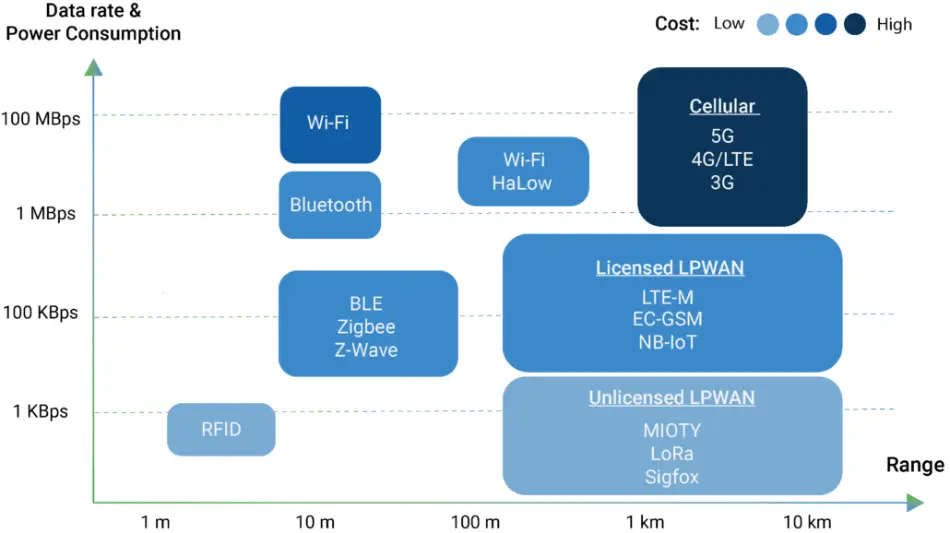
\includegraphics[width=1\textwidth]{pictures/lora/comparison-wireless-protocols.png}
    \caption{
        Comparison of data rate, power consumption and range between different wireless communication protocols.
        While \ac{LoRaWAN} has significantly lower data rates compared to cellular networks, its power consumption is also much lower.~\protect\cite{wang_comparison_2021}
    }\label{pic:wireless-protocols-comparison}
\end{figure}

While there are sensors that can be connected to the internet using Wi-Fi, ZigBee, \ac{LTE} and other, these technologies are not suitable for all use cases.

Deployments in remote or particularly spacious areas might need long-range protocols.
Likewise, sensors that are deployed in such areas can be hard to reach or placed apart by several hundred meters.
This makes low-power sensors that need to run on batteries for several years a necessity since replacing the batteries can be expensive or even impossible.

Wi-Fi is not suitable for battery-powered devices that are deployed in remote areas, as it requires relatively high power to operate and doesn't have much range.
ZigBee is also not suitable for battery-powered devices, as it is not designed for long distances and thus has a short range.
\ac{LTE} not suitable for battery-powered devices either as it requires a lot of power.
A rough comparison between selected wireless protocols can be seen in \cref{pic:wireless-protocols-comparison}~\cite{wang_comparison_2021}.

\subsection{\acf{RSSI}}\label{sec:rssi}

The \acl{RSSI} is a measure of the strength of a signal received by a device.
As far as this thesis is concerned, \ac{RSSI} values are measured in dBm since \ac{TTN}, the basis for all data used, uses this unit as well~\cite{the_things_industries_bv_data_2023}.

Different devices can have different \ac{RSSI} values for the same distance because of factors such as antennas with different gains.
Furthermore, \ac{RSSI} values can only function reliably when there is nothing blocking the signal between the transmitting and receiving stations, e.g.,\ if there is a \ac{LoS} between the sender and receiver.
The \ac{RF} signal can be blocked and thereby attenuated by walls, trees, or other objects.

\subsubsection{Correlation between \acs{RSSI} values and distance --- \acf{FSPL}}\label{sec:background-free-space-path-loss}

Usually, the higher the \ac{RSSI} value, the closer the sender is to the receiver since the signal is stronger when the radio waves have to travel a shorter distance~\cite{stutzman_antenna_1981}.
When using two non-directional (isotropic) antennas, there is a certain correlation between the distance between the sender and receiver and the \ac{RSSI} value.

The equation to calculate this so-called \acl{FSPL} in decibels can be seen in \cref{eq:fspl}~\cite[p. 1321]{whitaker_electronics_1996}.

\begin{equation}\label{eq:fspl}
    FSPL_{dB} = 20 \log_{10}\left(\frac{4 \pi d}{\lambda}\right)
\end{equation}

$d$ is the distance between sender and receiver, while $\lambda$ is the wavelength of the signal.

\begin{equation}\label{eq:wavelength-of-a-signal}
    \lambda = \frac{c}{f}
\end{equation}

To calculate the wavelength of a signal the formula seen in \cref{eq:wavelength-of-a-signal} is used, where $\lambda$ is the wavelength, $c$ is the speed of light, and $f$ is the frequency.
As the \ac{LoRa} modulation operates at \SI{868}{\mega\hertz} in the \ac{EU}, its wavelength can be calculated as $\lambda = \frac{299792458 \text{ m/s}}{868 \times 10^6 \text{ Hz}} \approx 0.345 \text{ m}$.

As an example, the \ac{FSPL} in \si{\decibel} for a distance of \SI{1}{\kilo\metre} (\SI{1000}{\metre}) with the \ac{LoRa} frequency can be calculated as follows: $20 \log_{10}\left(\frac{4 \pi \times 1000}{0.345}\right) \approx 91.23 \text{ dB}$.

\subsubsection{\acf{MPP}}\label{sec:multipath-propagation}

\begin{figure}[htbp]
    \centering
    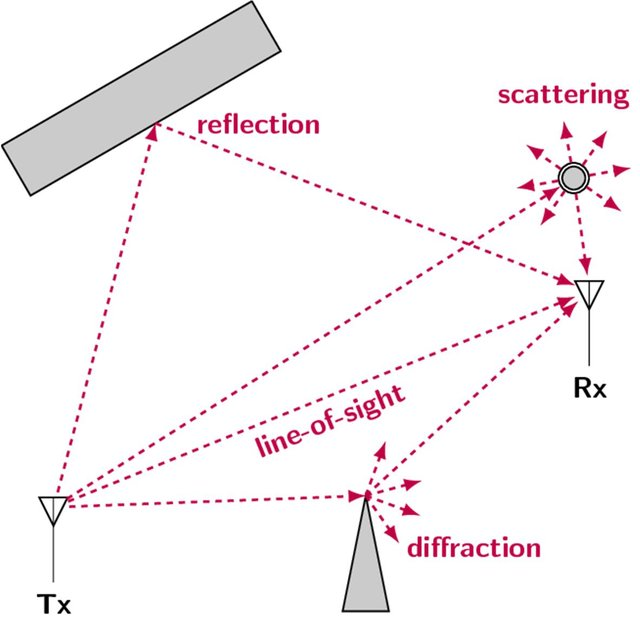
\includegraphics[width=0.4\textwidth]{pictures/diagrams_figures/multipath_propagation.jpg}
    \caption{
        Example for different kinds of \acf{MPP} of \ac{RF} waves.
        Notably, all of them make the signal travel time longer than direct \ac{LoS} would take.~\protect\cite{milosevic_key_2017}
    }\label{pic:figure_multipath_propagation}
\end{figure}

In addition to a signal reaching its destination directly, a \ac{RF} transmission phenomenon called \acf{MPP} can occur.
\acl{MPP} causes the \ac{RSSI} values to fluctuate even when neither the distance between the transmitter and receiver nor their antennas change~\cite[p. 136]{abdelfadeel_how_2019}.
This is because the signal can be reflected, diffracted, refracted and scattered and therefore take several paths (hence the term \ac{MPP}) as can be seen in \cref{pic:figure_multipath_propagation}.

\subsection{\acf{SNR}}

The \acf{SNR} is a measure of the strength of the signal compared to the noise in the signal.
Its formula is as follows:

\begin{equation}
    \text{SNR} = \frac{P_{signal}}{P_{noise}}
\end{equation}

A low \ac{SNR} indicates a signal that is influenced by a lot of noise.
The \ac{SNR} can be impacted by several environmental factors, such as the temperature and humidity of the air~\cite{jeftenic_impact_2020}.

\section{Terminology: \acs{LoRa} vs. \acs{LoRaWAN}}

\ac{LoRa} is a \ac{RF} communication modulation that offers a standard to send data packets over the air in a specific way.
The term \ac{LoRa} stands for \textbf{Lo}ng \textbf{Ra}nge~\cite{semtech_corporation_lora_2023}.
A rough explanation of its technical details can be found in \cref{sec:lora-modulation}.

\ac{LoRaWAN} is a network protocol that uses \ac{LoRa} as its physical layer.
It will be explained in more detail in \cref{sec:lorawan}.

\section{\acf{LoRa} modulation}\label{sec:lora-modulation}

The \ac{LoRa} modulation is also sometimes referred to as \ac{LoRa}\ PHY~\cite{chaudhari_understanding_2022}.
It uses several techniques to achieve long-range communication with low power consumption.
This section will explain some of its concepts that are relevant to this thesis.
However, it will not go into detail about the technical details of the modulation.

\Cref{sec:sf-snr-correlation} will explain how different \acfp{SF} interact with signals that have different \ac{SNR} values.

\subsection{Duty Cycle (in the \acs{EU} region)}\label{sec:duty-cycle}

\begin{figure}[htbp]
    \centering
    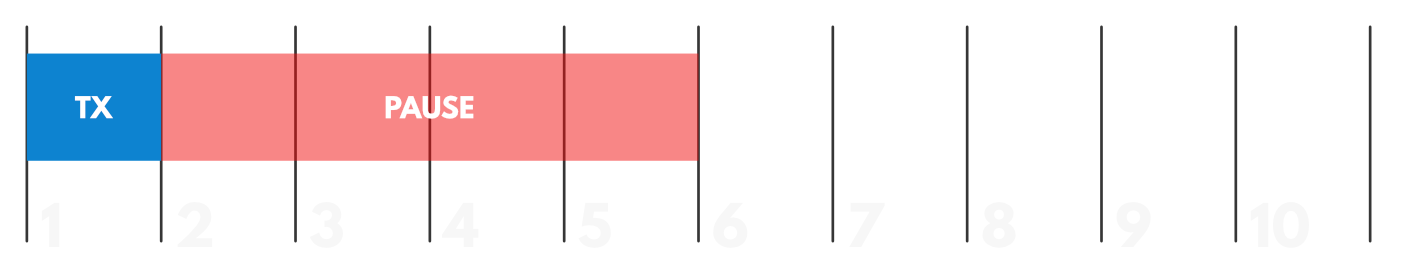
\includegraphics[width=.8\textwidth]{pictures/lora/duty-cycle-single-channel-off-air.png}
    \caption{
        Schematic example of duty cycle in \ac{LoRa}.
        For this example, the duty cycle is 20\%.~\protect\cite{the_things_industries_bv_duty_nodate}
    }\label{pic:lora-duty-cycle}
\end{figure}

In the \ac{EU} region, the duty cycle for transmissions in the 868 MHz band is limited to 1\%~\cite{etsi_etsi_2012}.
This means that a \ac{LoRa} device using a frequency band in this range may only transmit for 1\% of a given time slot.
If, for example, a device transmits data for 36 seconds, it must stay silent for the following 3,564 seconds, which is almost an hour.
It needs to stay silent for the rest of the time slot.

An example of a \ac{LoRa} duty cycle can be seen in \cref{pic:lora-duty-cycle}.
In this example, the duty cycle is 20\%.
The device that transmits for one block of time needs to stay silent for the next four time blocks before it can transmit again.

Luckily, LoRa packets are usually only a few bytes small and can thus be transmitted in a short amount of time, usually in a few milliseconds.

\subsection{\acf{CSS}}\label{sec:chirp-spread-spectrum}

\ac{LoRa} uses a technique called \acl{CSS} to transmit data with the possibility for error detection and correction.
This technique is important to be able to understand the \aclp{SF} in \cref{sec:spreading-factors}.

% TODO is this section even necessary? technical details seem to be out of scope for this thesis

\subsection{\acfp{SF}}\label{sec:spreading-factors}

The \ac{LoRa} modulation uses different \acfp{SF} to transmit data~\cite{the_things_network_spreading_2023}.
The \acl{SF} determines the chirp rate and thereby the data rate and range of the transmission.

There are six different \aclp{SF} available in the \ac{EU} region, ranging from \ac{SF}7 to \ac{SF}12.
\ac{SF}7 offers the highest data rate and the lowest range, while \ac{SF}12 offers the lowest data rate and the highest range.

\begin{figure}[htbp]
    \centering
    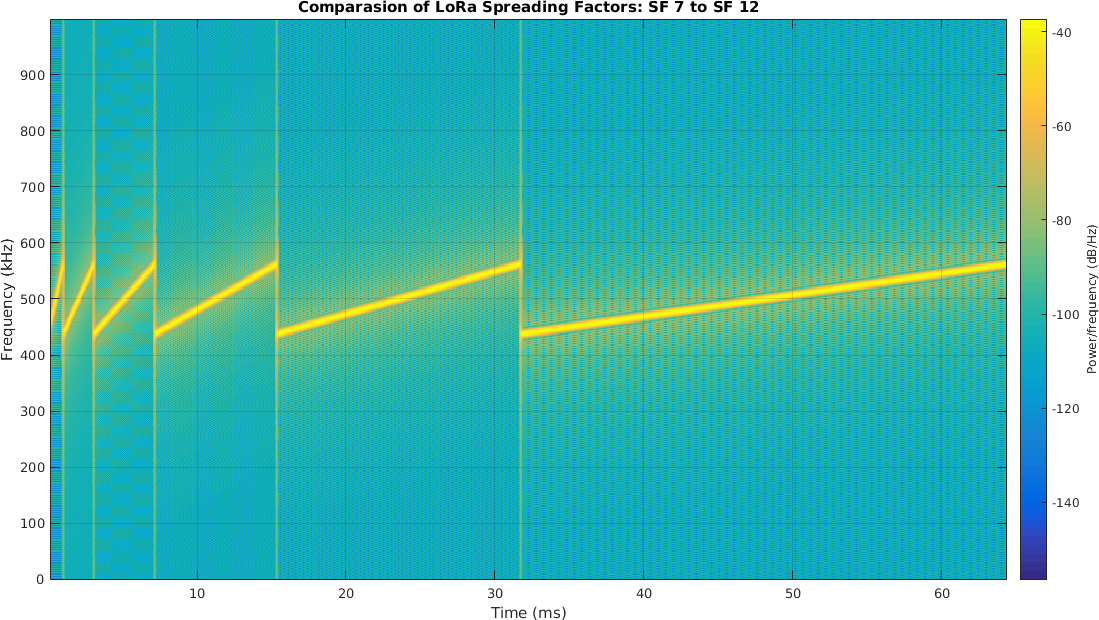
\includegraphics[width=0.7\textwidth]{pictures/lora/SF_Comparison_7_12.png}
    \caption{
        Comparison of \aclp{SF} \ac{SF}7 to \ac{SF} 12 in the time and frequency dimensions.
        The doubling of the transmission time between \aclp{SF} can be seen.\protect\cite{sakshama_ghoslya_lora_2017}
    }\label{pic:lora-sf-comparison}
\end{figure}

\Cref{pic:lora-sf-comparison} shows the difference between different \aclp{SF} in the time and frequency dimensions.
It shows that the higher the \ac{SF}, the longer the transmission takes.
In fact, the transmission time is proportional to $2^{\text{SF}}$~\cite{sakshama_ghoslya_lora_2017}.
This means that, for example, a transmission using \ac{SF}10 takes twice as long as a transmission using \ac{SF}9.

While a higher \ac{SF} means that data can be transmitted over a longer range, the transmission also takes longer.
Given the 1\% duty cycle in the \ac{EU} region mentioned in \cref{sec:duty-cycle}, this also means that using a higher \ac{SF} reduces the maximum amount of data that can be transmitted in any given timeframe.

Different \aclp{SF} also are orthogonal to each other, so they can be used at the same time without interfering with each other~\cite{the_things_network_spreading_2023}.

\subsubsection{Correlation of \acs{SF} and \acs{SNR}}\label{sec:sf-snr-correlation}

\aclp{SF} are important for this thesis because they interact with the\ac{SNR} values of a transmission.

% TODO write more = higher spreading factors mean that the SNR can be lower and the signal can still be recognized

\subsubsection{\ac{LoRa} transmission bit rates}

%  Explain how bit rates are affected by the duty cycle, spreading factor, bandwidth and coding rate

\subsection{Why use \acs{LoRa}?}

As can be seen in \cref{pic:wireless-protocols-comparison}, \ac{LoRa} is a good choice for devices that need to be able to operate battery-powered in remote locations for extended periods of time, as it has a long range and low power consumption.

A \ac{LoRa} node that transmits \SI{75}{\byte} of payload data every 2 hours can theoretically last up to 10 years on a single 1000 mAh battery~\cite{cheong_comparison_2017}.

\emph{LoRa Energy Calculator} is another piece of software that can be used to calculate the battery life of a \ac{LoRa} device by entering data such as payload size, periodicity of the data transmission and the battery type used~\cite{dramco_research_group_lora_2023}.
It calculates a ``worst case'' battery life of 6 years, 2 months and 1 week for a configuration with a payload size of 8 bytes, 1 hour of periodicity and a 2500 mAh AA type battery.
The ``best case'' scenario is rated at 17 years, 4 months and 1 week.
Best and worst case scenarios use different \aclp{SF} and \ac{TP} and also consider when the message is acknowledged.

\section{\acf{WAN}}

A \ac{WAN}, compared to a \acf{LAN} or \acf{MAN}, is a network that usually is not limited to one certain place, but connects multiple locations, across countries and continents~\cite[p. 2]{sadiku_fundamentals_2022}.
A well-known example of a \ac{WAN} is the Internet.

\begin{figure}[htbp]
    \centering
    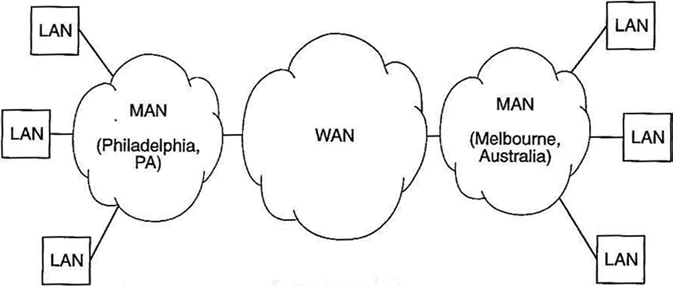
\includegraphics[width=.6\textwidth]{pictures/lorawan-structure/wan_diagram.png}
    \caption{
        An example connection between multiple \acfp{LAN} and \acfp{MAN} using a \acf{WAN} as a diagram.\protect\cite{sadiku_fundamentals_2022}
    }\label{pic:wan-diagram}
\end{figure}

\Cref{pic:wan-diagram} shows the connections between \acfp{LAN}, \acfp{MAN} and \acfp{WAN}.
\acp{WAN} consist of various \acp{MAN}.
\acp{MAN}, in turn, consist of various \acp{LAN}.

\subsection{\acf{LPWAN}}

% TODO Specifiy what a LPWAN is

While most \acp{WAN}, such as the Internet, typically have a high bandwidth and low latency, \acp{LPWAN}, on the other hand are designed to have ``low duty cycles, very low data rates, relatively longer latencies, low power consumption, and coverage over several kilometers''~\cite[p. 289]{kumar_connecting_2023}.
These factors make them more suitable for handling large amounts of sensors and actors that only need to transmit small amounts of data infrequently over long distances.

\begin{figure}[htbp]
    \centering
    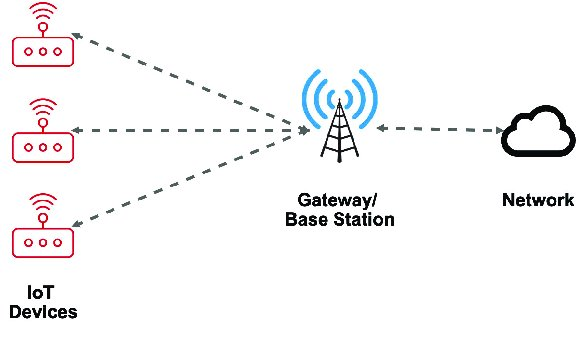
\includegraphics[width=.5\textwidth]{pictures/lorawan-structure/lpwan_network_structure.jpg}
    \caption{
        A simple diagram of a \ac{LPWAN} network structure.
        The connections between the entities can be seen.\protect\cite{fernandez_assessing_2020}
    }\label{pic:lpwan-diagram}
\end{figure}

\Cref{pic:lpwan-diagram} shows the structure of a \ac{LPWAN} network.
Multiple \ac{IoT} devices connect to gateways or base stations.
Those gateways are in turn connected to the internet or a larger network via a backhaul connection.

\section{\acf{LoRaWAN}}\label{sec:lorawan}

\begin{figure}[htbp]
    \centering
    
\includegraphics[width=.3\textwidth]{pictures/logos/LoRaWAN_Logo.eps}
    \caption{
        \ac{LoRaWAN} logo~\protect\cite{lora_alliance_francais_2022}
    }
\end{figure}

\ac{LoRaWAN} uses the \ac{LoRa} wireless communication protocol to create a \ac{LPWAN} where multiple devices can communicate with each other over long distances.
It defines a secure way to transfer packets from the end devices to the application server by enforcing \ac{E2EE}.
This section will explain the structure of a \ac{LoRaWAN} network and its inner workings.

\subsection{\acs{LoRaWAN} network architecture}

\begin{figure}[htbp]
    \centering
    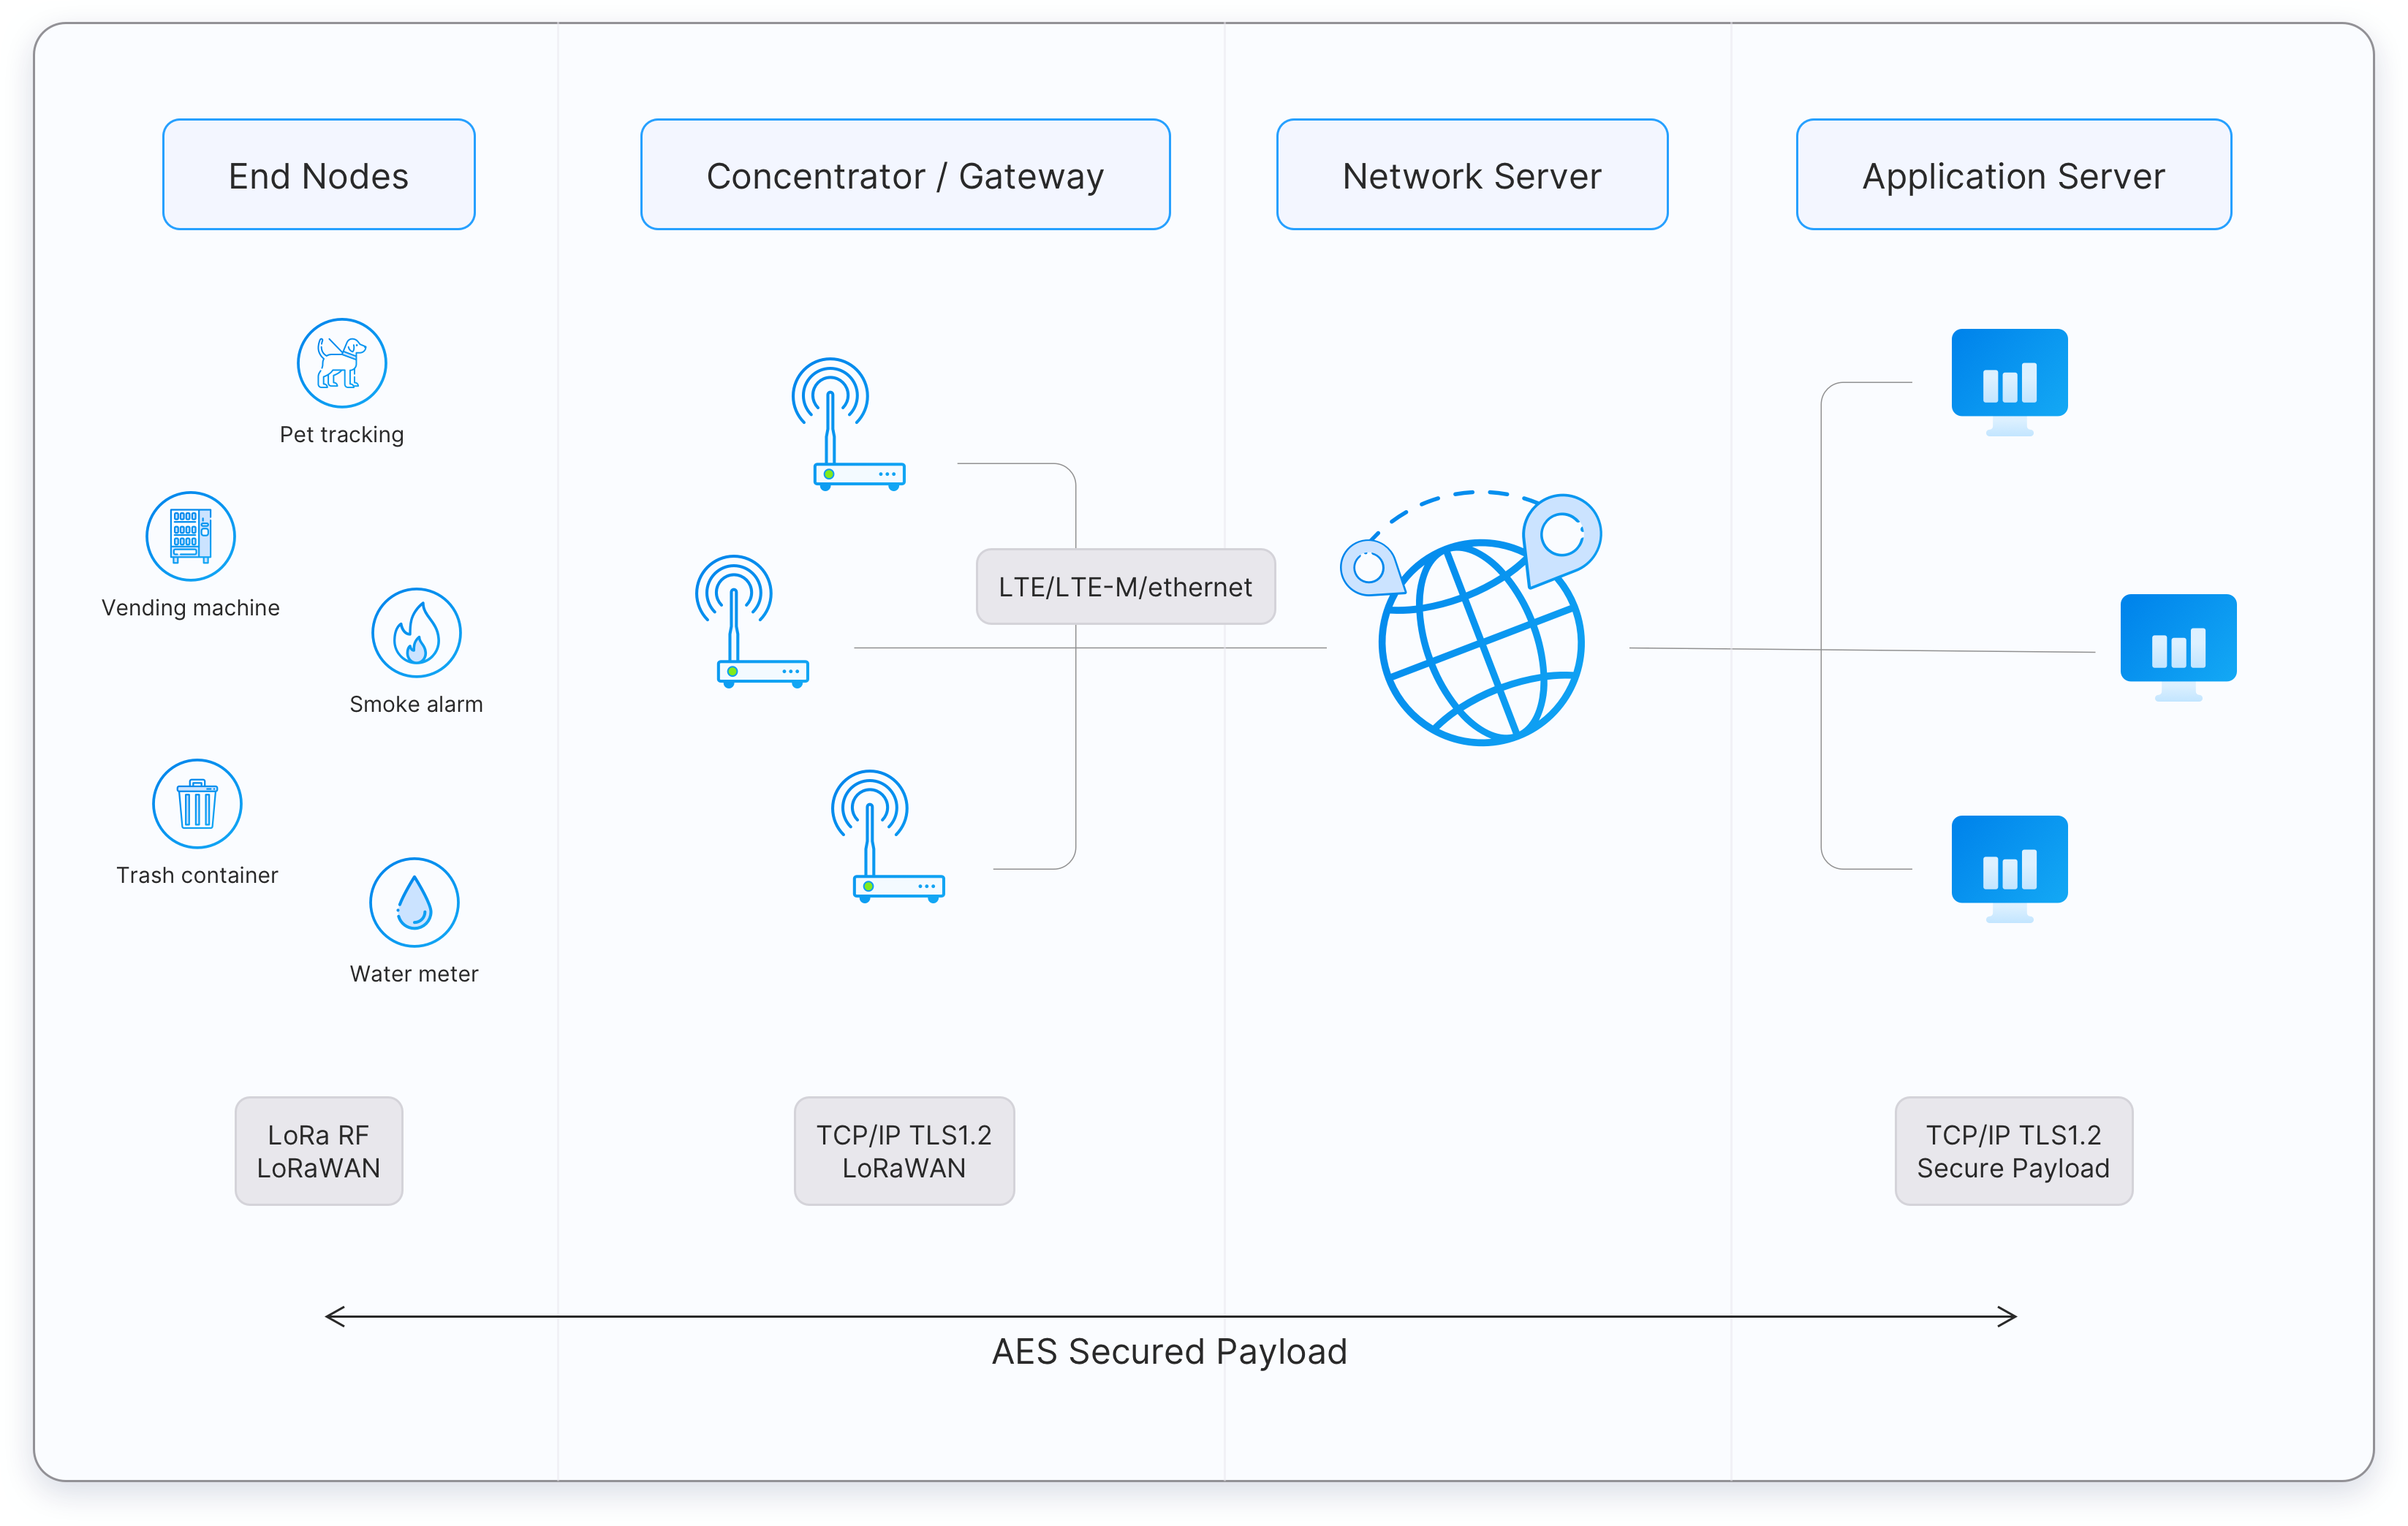
\includegraphics[width=1\textwidth]{pictures/lorawan-structure/lorawan-architecture.png}
    \caption{
        The structure of a \ac{LoRaWAN} network.~\protect\cite{the_things_industries_bv_lorawan_nodate}
    }\label{pic:lorawan-network-structure}
\end{figure}

The \ac{LoRaWAN} network architecture, as seen in \cref{pic:lorawan-network-structure} consists of four main components~\cite[p. 8]{lora_alliance_inc_lorawan_2017}:

\begin{itemize}
    \item The end nodes (also called end devices),
    \item the gateways (also called concentrators or base stations),
    \item the \acf{LNS}, and
    \item the \acfp{AS}.
\end{itemize}

\ac{LoRaWAN} data rates typically range from 0.3 kbps to 50 kbps, depending on the region and the \ac{LoRa} modulation used~\cite[p. 8]{lora_alliance_inc_lorawan_2017}.

\subsection{Gateways}

\begin{figure}[htbp]
    \centering
    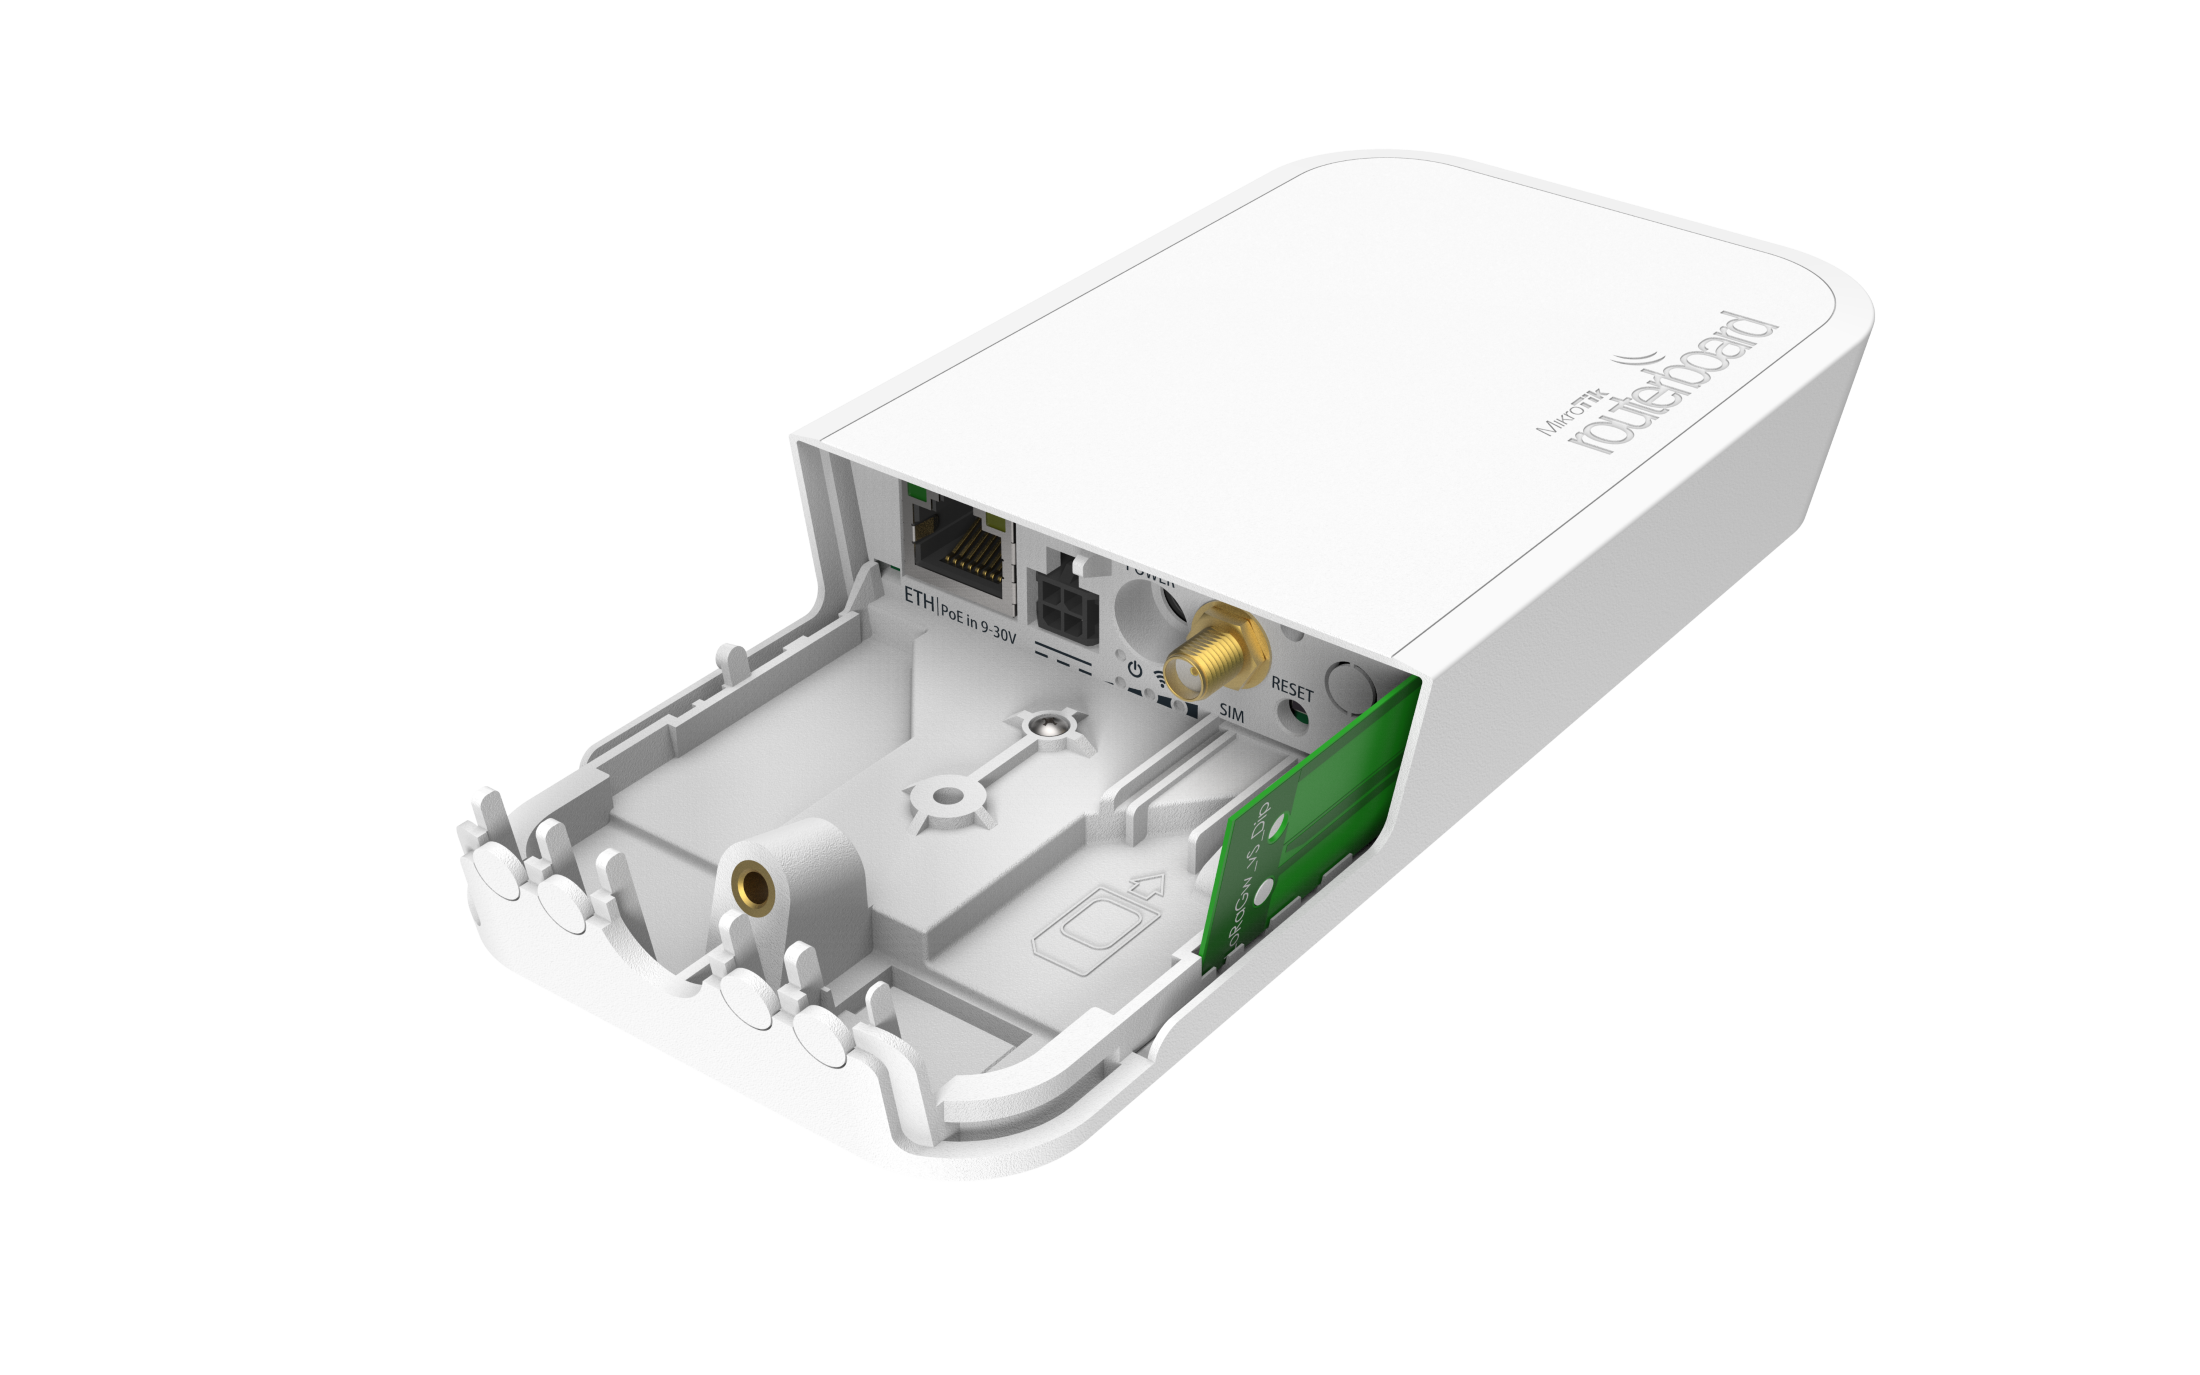
\includegraphics[width=.6\textwidth]{pictures/hardware/gateways/mikrotik-lr8-kit.png}
    \caption{
        A MikroTik wAP LR8 kit \ac{LoRaWAN} Gateway.
        This was one of the gateways used during this thesis.~\protect\cite{the_things_industries_bv_lorawan_nodate}
    }\label{pic:mikrotik-lr8-kit-gateway}
\end{figure}

A \ac{LoRa} gateway is a device that receives \ac{LoRa} packets (usually from \ac{LoRa} nodes/end devices) and forwards them to the \ac{LoRaWAN} server.

\ac{LoRa} gateways are usually based on a \ac{LoRa} concentrator, which is a \ac{RF} module that receives \ac{LoRa} packets and forwards them to the gateway's \ac{CPU} using a serial interface.
The \ac{CPU} processes the incoming data and forwards the packets to the \ac{LoRaWAN} server.

To achieve the connection to the \ac{LoRaWAN} server, the gateway needs to be connected to the internet.
This connection is also called \emph{backhaul}.
The most widely used methods to realize this are Ethernet/\ac{LAN}, Wi-Fi and \ac{LTE} connections~\cite{the_things_industries_bv_lorawan_nodate}.

One example of a gateway used during this thesis and therein installed in Furtwangen is the \emph{MikroTik wAP LR8 kit}, as seen in \cref{pic:mikrotik-lr8-kit-gateway}.
This gateway is specified as suitable for outdoor usage, making it a good choice for the deployment in Furtwangen on top of (among others) the roof of the student dorm \ac{GHB}.

\begin{figure}[htbp]
    \centering
    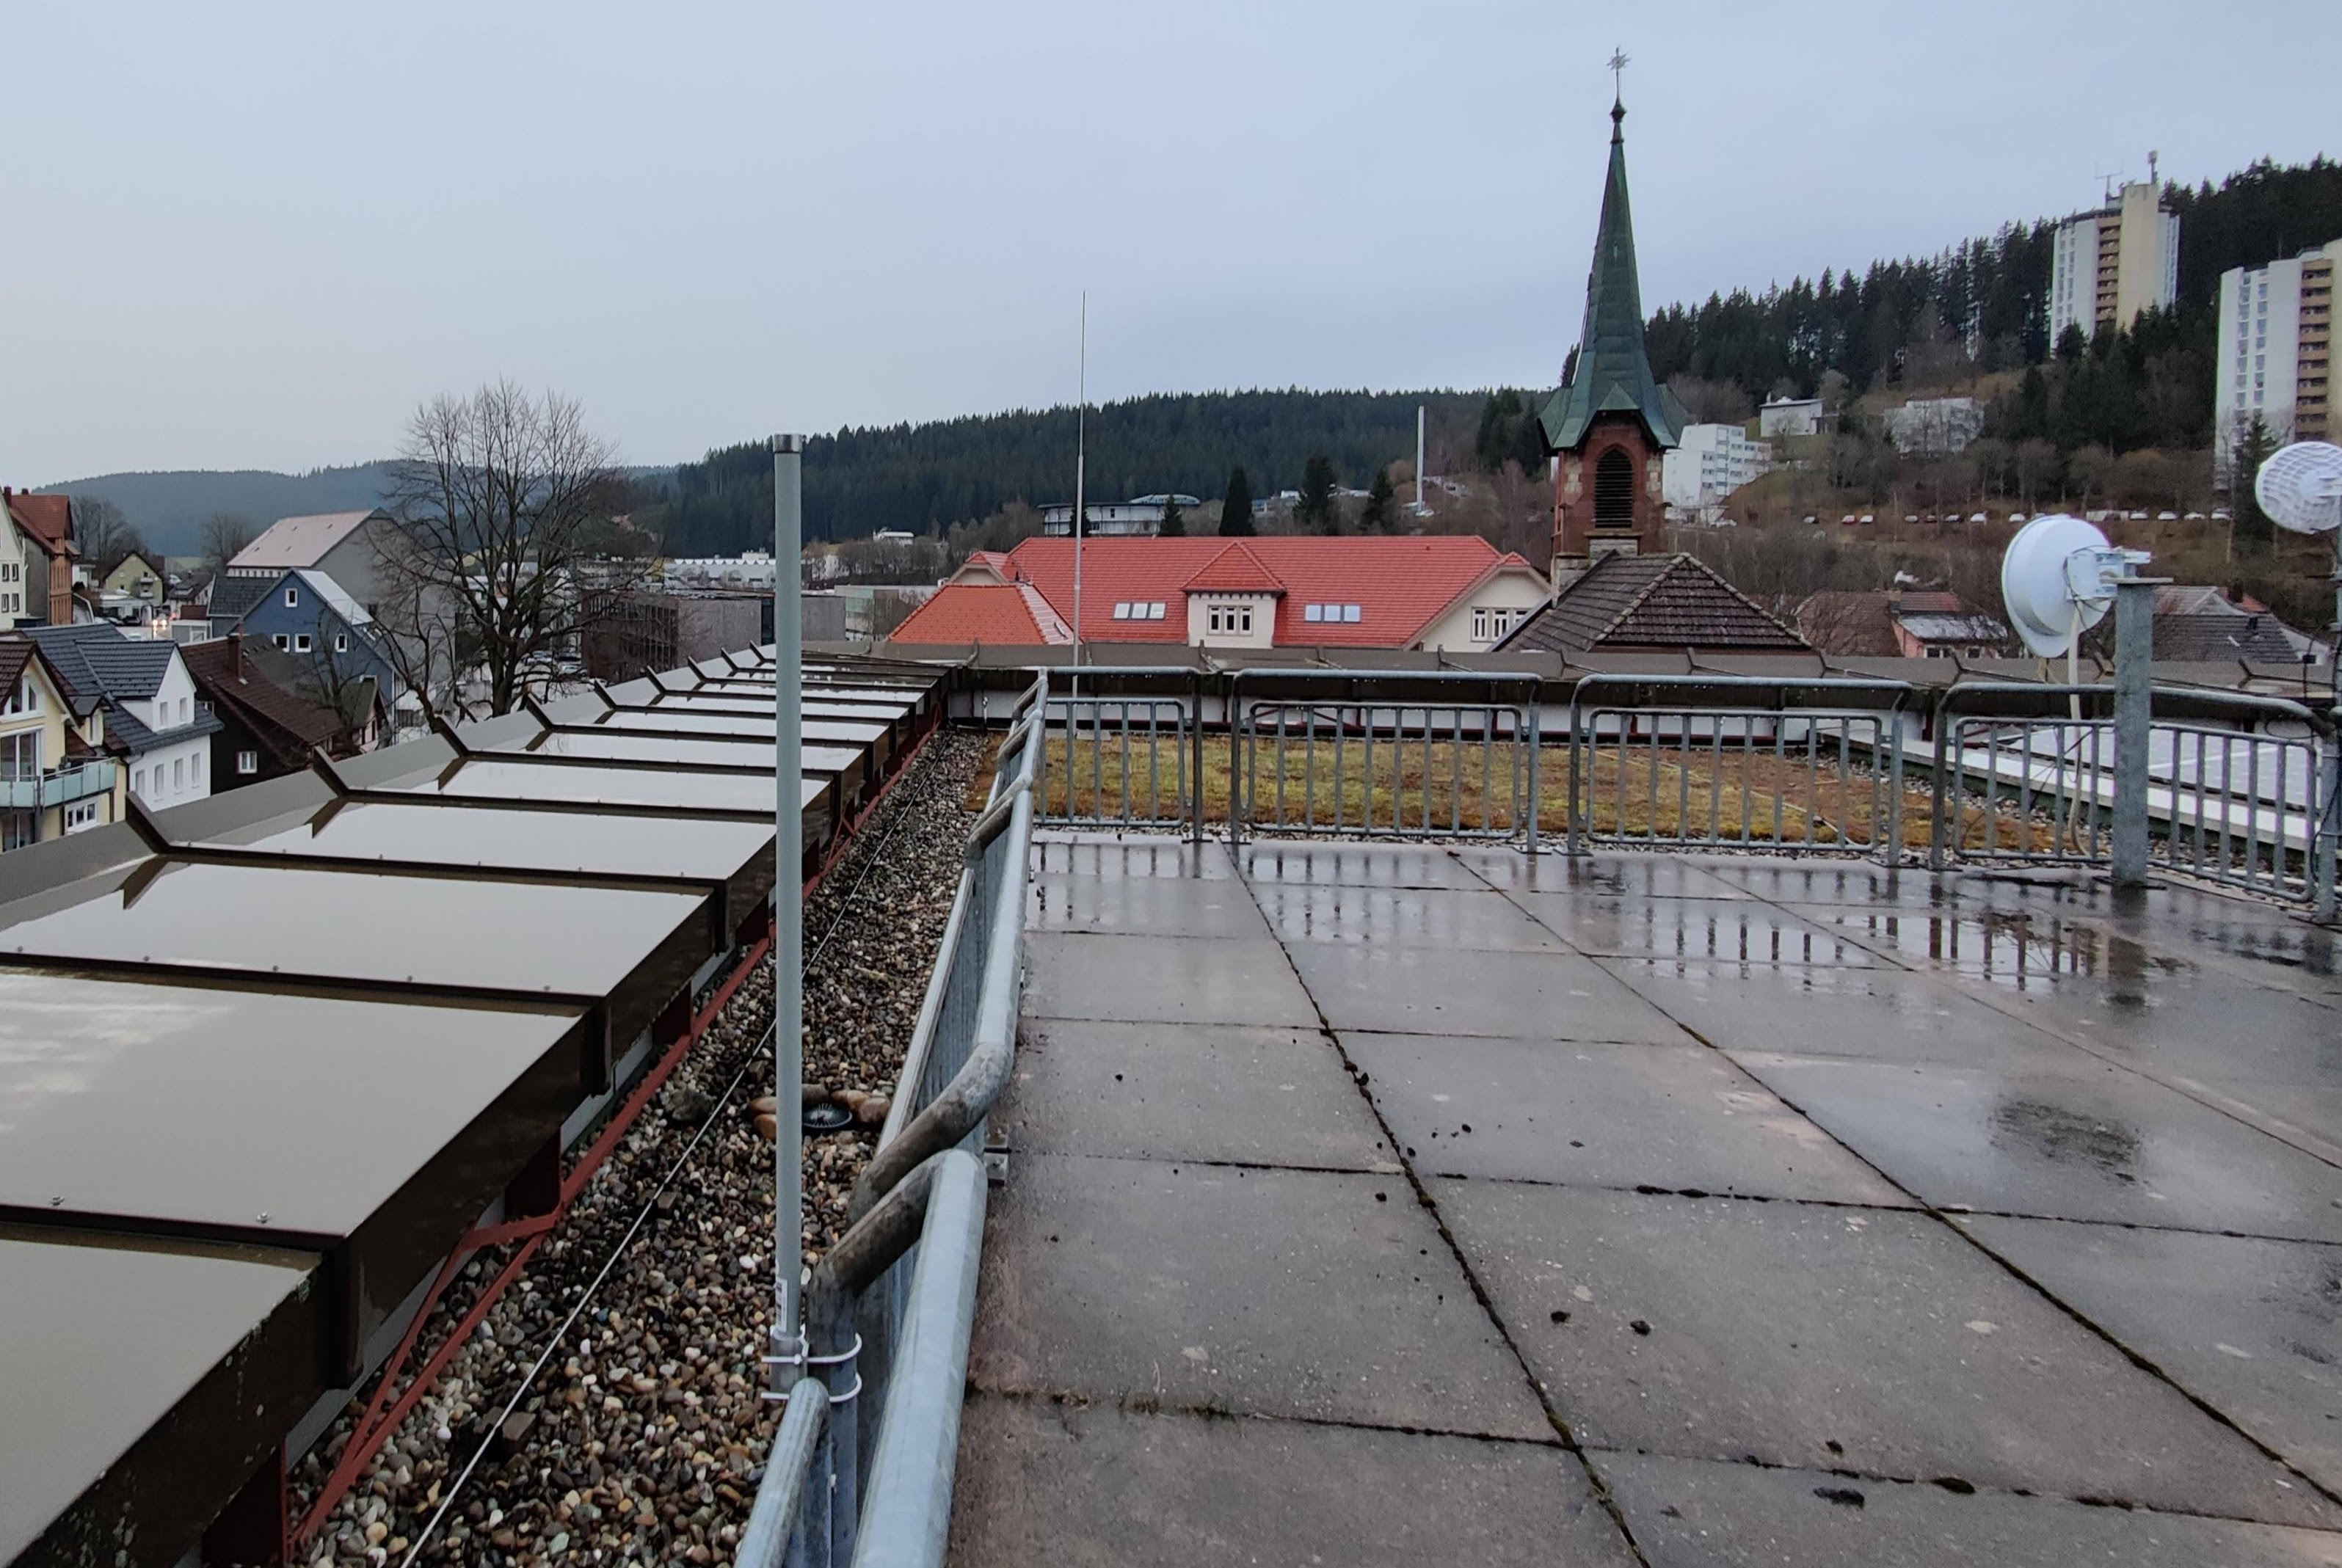
\includegraphics[width=0.6\textwidth]{pictures/hardware/gateway-deployment/mikrotik-antenna-c-building.jpg}
    \caption{
        A MikroTik antenna installed on top of the \ac{HFU} C building.
        The exposed position of the roof in the valley where Furtwangen is located can be seen.
        In the background, on the right, the two buildings of the \ac{GHB} dormitories are visible.
    }\label{pic:mikrotik-antenna-c-building}
\end{figure}

While gateways like these usually have a built-in antenna, their range is only sufficient for covering small to medium-sized buildings or areas.
It is, however, also possible to use external antennas if it is necessary to cover a much larger area as was the case in this thesis since a medium to long range localization of \ac{LoRa} nodes was the goal.
While there are many options for external antennas, in the case of the MikroTik gateway, the decision was made to also use the external \ac{LoRa} antenna supplied by MikroTik, as it is specifically designed for the MikroTik gateway and thus should be a good match.
The deployment of this antenna on top of the \ac{HFU} C building is shown in \cref{pic:mikrotik-antenna-c-building}.

\subsection{Data Transmission}

In LoRaWAN, data transmissions to and from the end nodes are called \emph{uplink} and \emph{downlink}, respectively~\cite[p. 12]{lora_alliance_inc_lorawan_2017}.

Uplinks are relayed to the network server by one or more gateways from the end node.
Downlinks, however, are only sent from the network server to the end node using a single gateway.
\subsection{Device Classes}

\ac{LoRaWAN} defines three classes of devices that offer different variations of the trade-off between power consumption and data rate/availability~\cite[p. 10]{lora_alliance_inc_lorawan_2017}.

\subsubsection{Class A}

\begin{figure}[htbp]
    \centering
    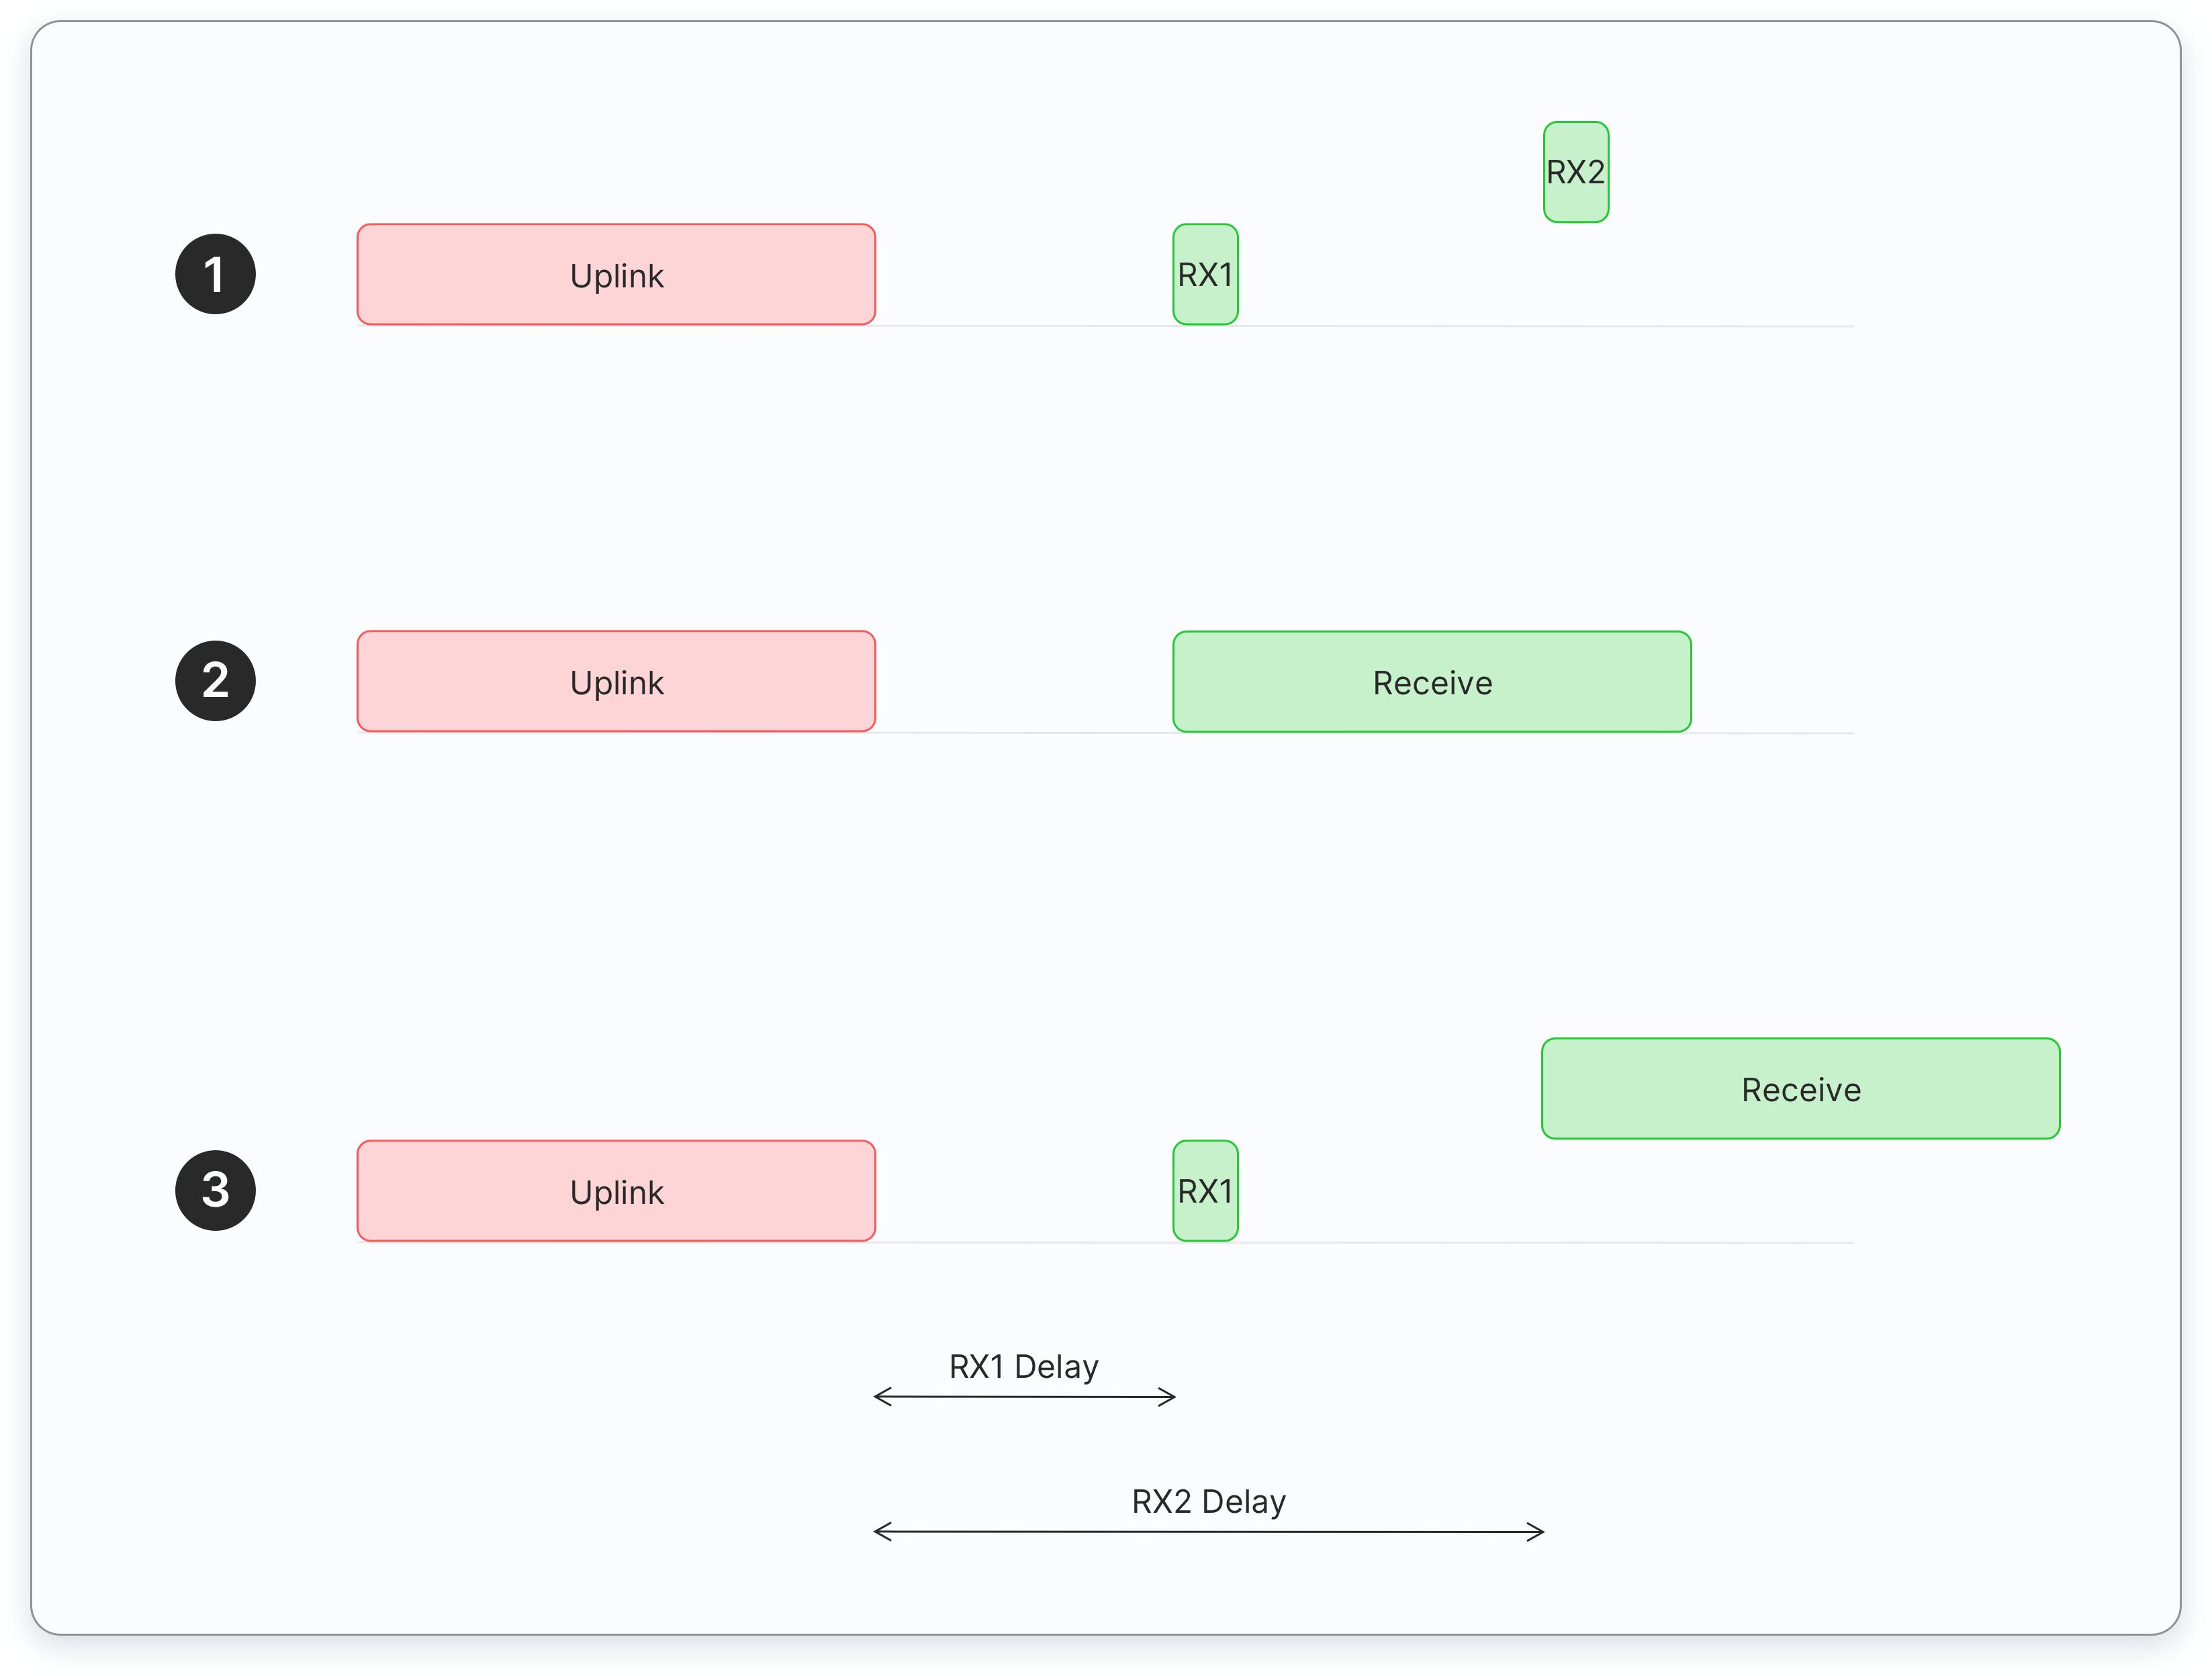
\includegraphics[width=1\textwidth]{pictures/device-classes/class-a.png}
    \caption{
        A schema of a \ac{LoRaWAN} Class A device communication.
        The two receive windows (RX1 and RX2) are visible.~\protect\cite{the_things_industries_bv_device_nodate}
    }\label{pic:lorawan-device-class-a-schema}
\end{figure}

Class A is used for devices that need to consume as little power as possible.
Every \ac{LoRaWAN} device must support the Class A mode~\cite[p. 11]{lora_alliance_inc_lorawan_2017}.
A communication in Class A is always initiated by the end device itself.

Bidirectional communication is possible in Class A through the use of two downlink receive windows during which it is possible for the \ac{LNS} to send data to the device.
This can be seen in \cref{pic:lorawan-device-class-a-schema}.
This also makes it impossible for the \ac{LNS} to send data to the device at any other time.

Class A consumes the least amount of power of the three classes, since the devices itself may specify when and how often they want to communicate with the \ac{LNS}.

\subsubsection{Class B}

\begin{figure}[htbp]
    \centering
    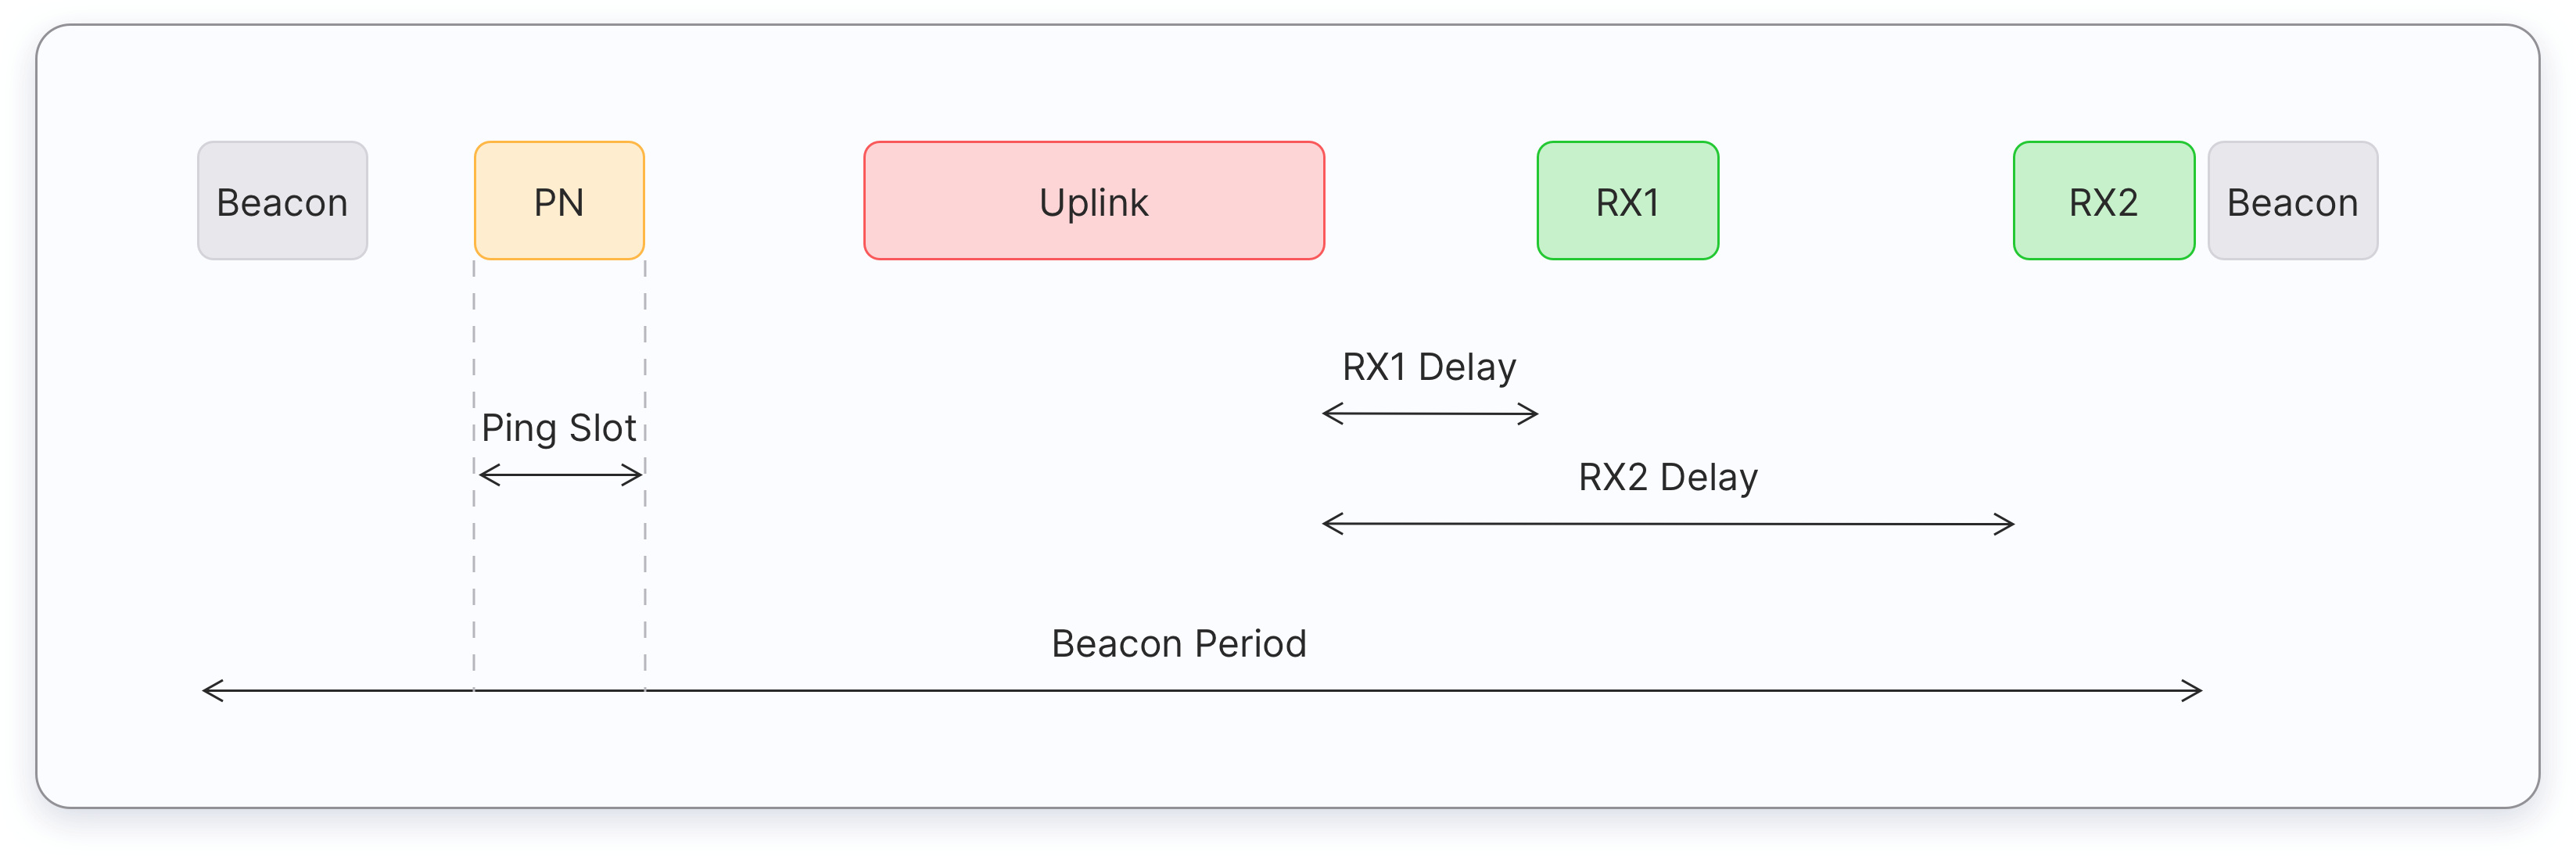
\includegraphics[width=1\textwidth]{pictures/device-classes/class-b.png}
    \caption{
        A schema of a \ac{LoRaWAN} Class B device communication.
        The additional ping slots where the end device is reachable by gateways can be seen.~\protect\cite{the_things_industries_bv_device_nodate}
    }\label{pic:lorawan-device-class-b-schema}
\end{figure}

In addition to class A, class B devices are also able to receive downlink messages from the \ac{LNS} during dedicated downlink receive windows.
In order to realize this without the need for a per-device \ac{RTC}, class B devices receive time synchronized beacons from the gateways.
The communication schema for class B devices can be seen in \cref{pic:lorawan-device-class-b-schema}.

These scheduled downlink windows result in a higher power consumption for class B devices, since those need to be awake during these windows.

\subsubsection{Class C}

\begin{figure}[htbp]
    \centering
    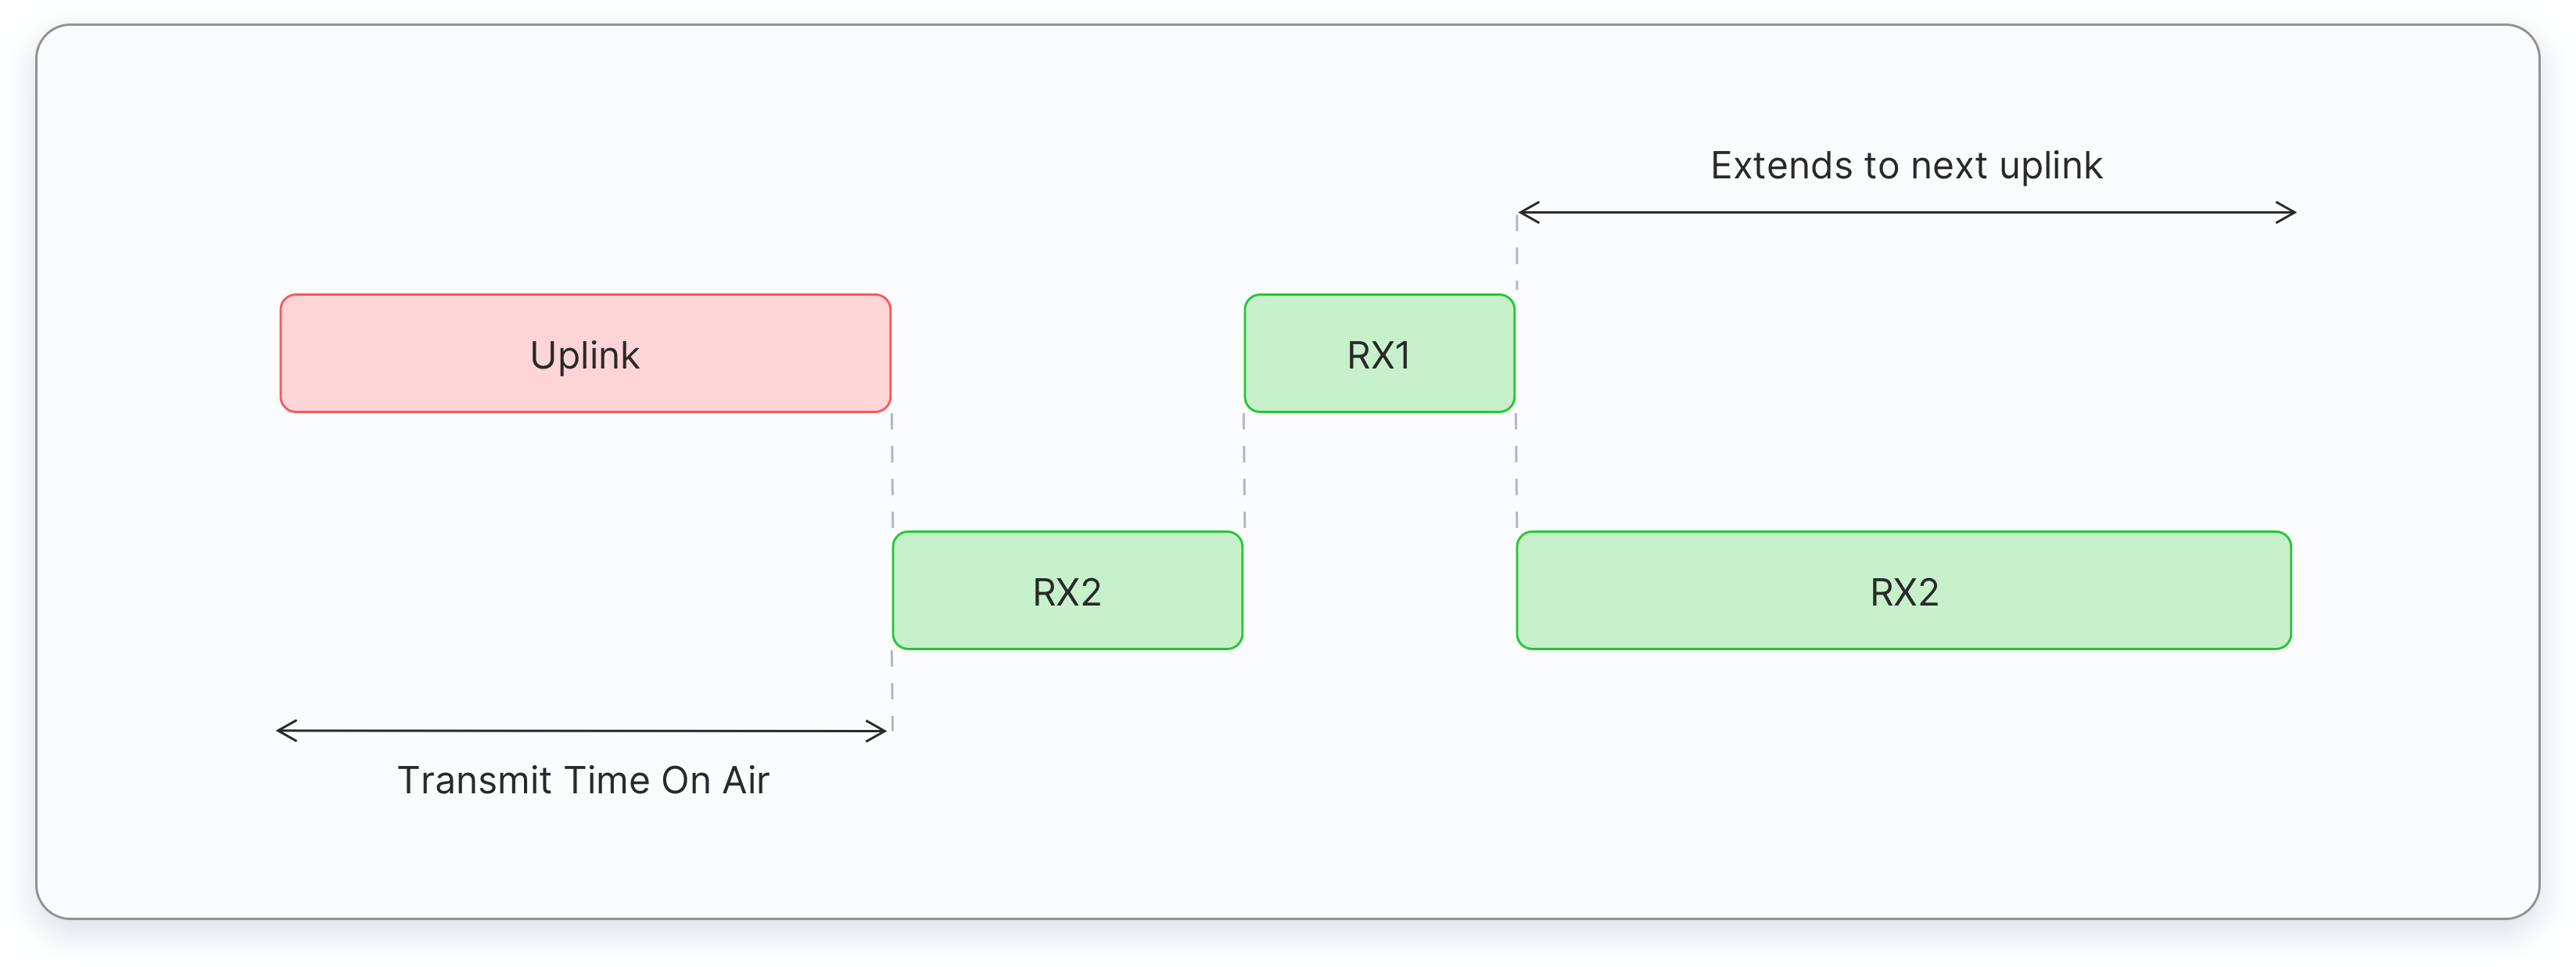
\includegraphics[width=1\textwidth]{pictures/device-classes/class-c.png}
    \caption{
        A schema of a \ac{LoRaWAN} Class C device communication.
        The RX2 window is kept open between uplink transmissions to allow gateways to reach the end device at any time while no uplinks are occurring.~\protect\cite{the_things_industries_bv_device_nodate}
    }\label{pic:lorawan-device-class-c-schema}
\end{figure}

Class C devices, when not currently transmitting an uplink message, are always listening for downlink messages from the \ac{LNS}.
In essence, they keep the downlink windows as specified in class B open all the time as seen in \cref{pic:lorawan-device-class-c-schema}.

Devices in class C consume the most power, since they are always listening for downlink messages.
The fact that they are always reachable by the \ac{LNS} also makes them the most suitable for applications that require a high data rate or a reliable accessibility via downlink.

\subsubsection{Conclusion}

As far as this thesis was concerned, only Class A devices were used.
This is because Class B and C use significantly more power than class A because they keep their radio on for extended periods of time, which is a problem for battery-powered devices.

In their paper ``Comparison of LoRaWAN Classes and their Power Consumption'', Cheong et al.\ show that a device in Class C would need a battery around 19 times larger than a Class A device to achieve the same battery life with a packet size of 115 bytes and a transmission interval of 1 hour~\cite{cheong_comparison_2017}.
As mobile devices that have the need to be located are usually battery-powered, class A is the most viable option for them.

The geolocation methods evaluated in this thesis work with any \ac{LoRaWAN} device class.
While using Class C would mean that devices could actually be asked directly for their location, using Class A devices is usually the better choice due to the lower power consumption.

\subsection{Data security}

The security of the data sent is a major concern when talking about \ac{IoT} protocols.
\ac{LoRaWAN} uses \ac{AES} based \acf{E2EE}.
Each end device usually has a unique 128-bit \ac{AES} key that is used for payload encryption~\cite{lora_alliance_inc_lorawan_2017-1}.

This \ac{E2EE} also makes \ac{LoRaWAN} packages secure against replay attacks, since a so-called \ac{MIC} is determined using the frame data~\cite{lora_alliance_inc_lorawan_2017-1}.

\section{\acf{TTN}}

\ac{TTN} provides a free to use \ac{SaaS} \ac{LNS} that supports a global community of people building \ac{LoRaWAN} applications.
Its source code, named \ac{TTS}, is also available on GitHub under the Apache 2.0 license~\cite{the_things_network_thethingsnetworklorawan-stack_2023}.

\begin{figure}[htbp]
    \centering
    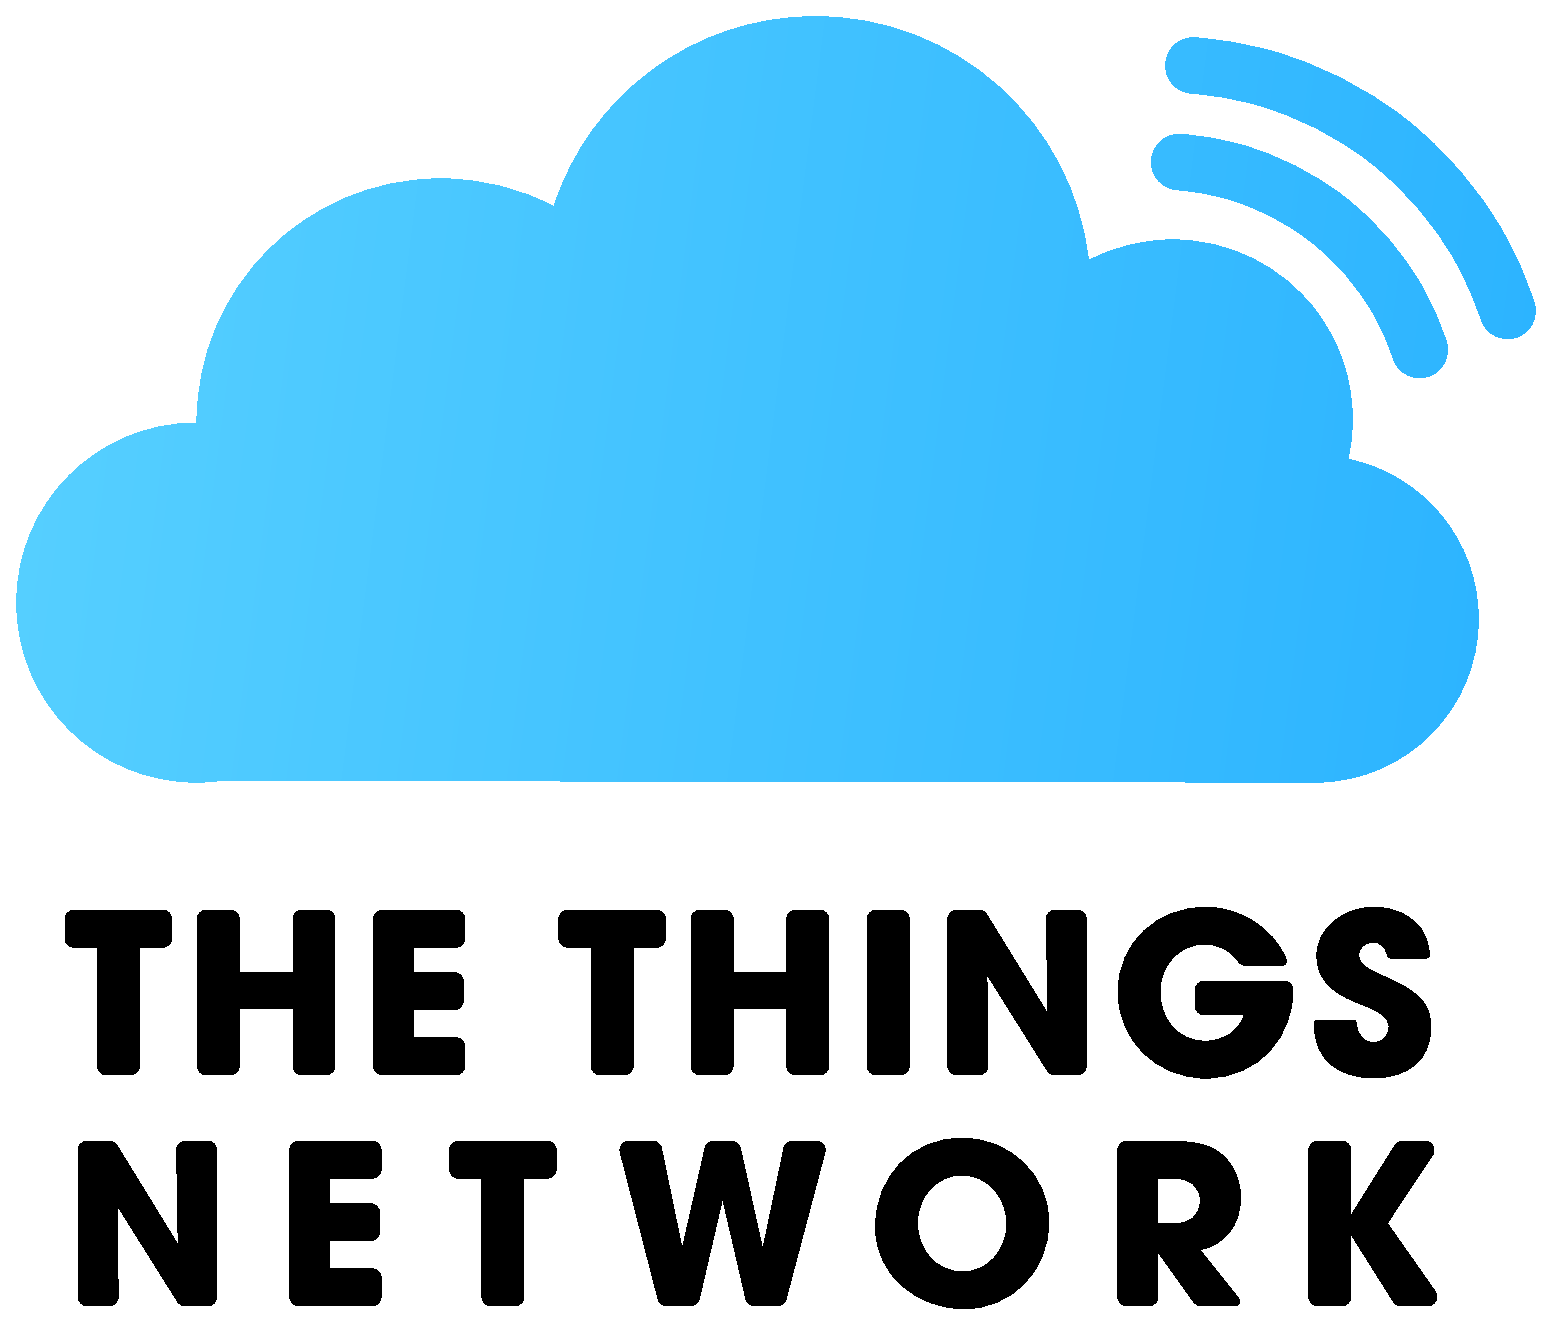
\includegraphics[width=0.3\textwidth]{pictures/logos/TTN-logo.eps}
    \caption{\acf{TTN} logo~\protect\cite{the_things_industries_bv_quick_nodate}}
\end{figure}


While, officially, it is called \emph{\acl{TTS} Community Edition} since 2021, it is still commonly referred to as \acf{TTN}~\cite{the_things_industries_bv_what_2022}.
Its users provide \ac{TTN} with gateways that other users can use, making it a decentralized and crowdsourced \ac{LoRaWAN} network.

\subsection{Receiving packets from \acs{LoRaWAN} Gateways}

Gateways can forward \ac{LoRaWAN} packets that it receives to the \ac{LNS} in two major ways:

\subsubsection{\acf{SUPF}}

The \ac{SUPF} is a piece of software used to connect \ac{LoRa} gateways to the \ac{LNS}~\cite{the_things_industries_bv_semtech_2022}.
The \ac{SUPF} relays \ac{LoRaWAN} packets that it receives from its connected \ac{LoRa} concentrator to the \ac{LNS} using the \ac{UDP} protocol.

It may be configured using JSON files such as \lstinline{global_conf.json} and \lstinline{local_conf.json}.

\ac{TTN} marked the \acl{SUPF} as deprecated, since it ``has many security and scalability drawbacks``~\cite{the_things_industries_bv_semtech_2022}.
It is advised to use the \acl{LBS} protocol instead.

\subsubsection{\acf{LBS}}

Since \ac{TTN} v3, using the \ac{TCP}-based \acl{LBS} protocol is recommended over the \ac{SUPF} to connect gateways to the \ac{LNS}~\cite{the_things_industries_bv_semtech_2022}.

\begin{figure}[htbp]
    \centering
    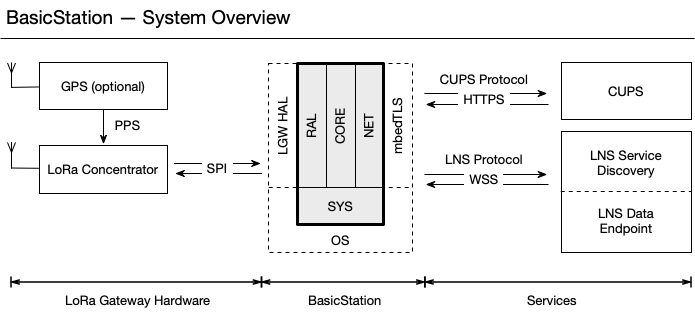
\includegraphics[width=0.9\textwidth]{pictures/lorawan-structure/lora-basics-station-structure.png}
    \caption{
        A schema of communications from a gateway and a \ac{LNS} using \acf{LBS}.
        The \ac{CUPS} service can be seen in the top right.~\protect\cite{semtech_lora_developer_portal_lora_2022}
    }\label{pic:lora-basics-station-schema}
\end{figure}

\ac{LBS} uses \ac{TLS}-encrypted \ac{TCP} connections with token-based authentication to relay \ac{LoRaWAN} packets to the \ac{LNS}~\cite{the_things_industries_bv_lora_2022}.

The two main components of \acl{LBS} are the \ac{LNS} connection itself as well as the \acf{CUPS}.
The communication schema can be seen in \cref{pic:lora-basics-station-schema}.

The \ac{LNS} uses \ac{WSS} for communication and is responsible for handling the \ac{LoRaWAN} packets whereas the \acl{CUPS} is responsible for handling the configuration of the gateways.

While \ac{CUPS} is not strictly necessary for sending actual \ac{LoRaWAN} packets, it simplifies the management of gateways and their configuration.
It communicates using \ac{TLS}-encrypted \ac{TCP} (\ac{HTTPS}) connections with token-based authentication.
When a gateway is configured with \ac{CUPS}, it will automatically receive its configuration from the \ac{LNS} and be authenticated to work with it~\cite{the_things_industries_bv_lora_2022}.

\subsection{Web Interface and Device/Gateway Management}\label{sec:web-interface-and-device-gateway-management}

\ac{TTN} provides a web interface for managing devices and gateways that are registered to the network.
It also provides a \ac{REST} \ac{API} for managing devices and gateways programmatically.

End devices are grouped into \emph{applications} that can be used to manage \ac{LoRaWAN} end devices that belong to a bigger project or device group.

In this thesis, an application was used to group the \ac{LoRaWAN} \ac{GPS} trackers that were used for data collection.

\subsection{Forwarding data from \acf{TTN} to \acfp{AS}}\label{sec:forwarding-data-from-ttn-to-as}

To transmit data from \ac{TTN} to an \ac{AS}, \ac{TTN} provides \emph{integrations}~\cite{the_things_network_integrations_2021}.
\ac{TTN} offers several integrations for different cloud \acp{AS} such as \ac{AWS} IoT Core and Microsoft Azure IoT Hub.
It also provides a generic \ac{HTTP} webhook integration that can be used to forward data to any \ac{HTTP} or \ac{HTTPS} endpoint.

Additionally, \ac{TTN} provides a MQTT integration, which can send data to an MQTT broker.
MQTT is a widely used lightweight publish-subscribe messaging protocol that is often used in \ac{IoT} applications~\cite{mqtt_mqtt_2022}.
It is not used in this thesis, so it will not be discussed further.

\ac{TTNM}, the service that was used to collect geolocation data from \ac{LoRaWAN} devices in this thesis, uses a webhook integration to collect data from \ac{TTN}.
This is explained in more detail in \cref{sec:ttm-data-collection}.

Integrations are usually managed on a per-application basis.
This means that different integrations can be used for different applications.

\subsection{Alternatives to \acf{TTN}}

While anyone can use \ac{TTN} for free as a cloud-hosted \ac{SaaS}, it is not the only \ac{LNS} available.
\ac{TTN} can also be self-hosted, for example using Docker, using the open-source \ac{LNS} \emph{The Things Stack}~\cite{the_things_network_host_2023}.

There are also several other \acp{LNS} that can be used to build a private \ac{LoRaWAN} network.

\emph{LORIOT} is \ac{TTN} --- it has a public community instance that acts similar to the \ac{SaaS} version of \ac{TTN}, and it also offers a self-hosted version~\cite{loriot_ag_loriot_2023}.
It is, contrary to \ac{TTN}, not open-source.

Another well-known \ac{LNS} is \emph{ChirpStack}, which is open-source and can be self-hosted~\cite{chirpstack_chirpstack_2023}.
Contrary to \ac{TTN}, it is not a \ac{SaaS} and does not offer a public community instance.

\section{\acf{TTNM}}

\acf{TTNM} was created by engineer JP Meijers in 2015~\cite{linkedin_23_nodate}.
He first created it as a personal project to map the range of his own \ac{LoRaWAN} gateway.
However, the project has since been expanded to map the coverages of almost all gateways registered in the public \ac{TTN} network~\cite{the_things_network_jp_2018}.

\subsection{Data collection}\label{sec:ttm-data-collection}

\acl{TTNM} works by using \ac{LoRaWAN} nodes with \ac{GPS} modules that send their location to the \ac{TTN} network via uplink messages.
Alongside the location information, those nodes' messages that are processed by \ac{TTN} also include information about which gateways received them.

Hence, \acl{TTNM} can use the information about which gateways received the message and the location information of the nodes' \ac{GPS} modules.
This is done by means of a \emph{webhook} that sends the data to an endpoint of the \acl{TTNM} \ac{API} whenever a node sends a message to the \ac{TTN} network as has been explained in \cref{sec:forwarding-data-from-ttn-to-as}.
With this data, it can build a map displaying the coverage of \ac{LoRaWAN} gateways in the \ac{TTN} network.

\subsection{Frontend data views}

\begin{figure}[htbp]
    \centering
    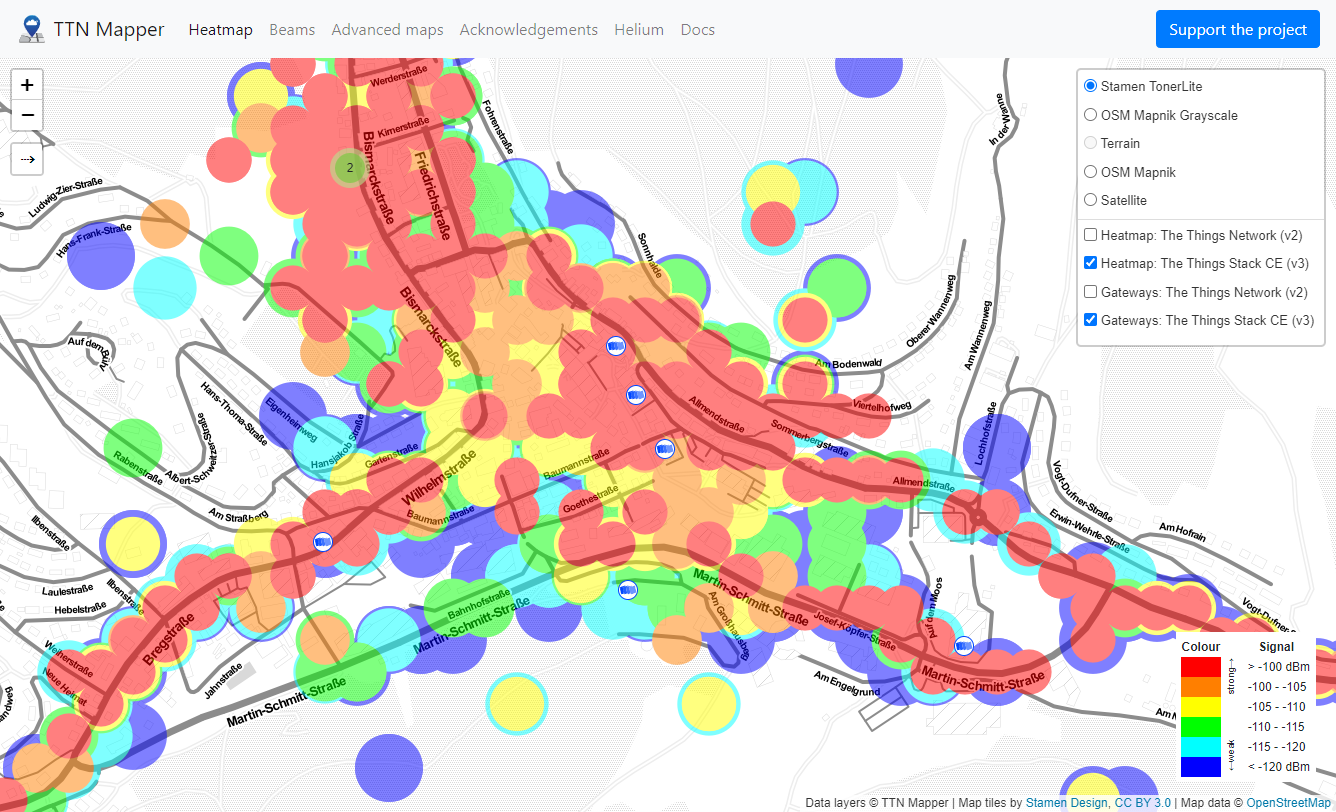
\includegraphics[width=1\textwidth]{pictures/ttn-mapper/heatmap_with_gateways.png}
    \caption{
        A screenshot of \ac{TTNM}'s \emph{heatmap} view of the Furtwangen area.
        The heatmap shows places where strong signals from \ac{LoRaWAN} gateways were recorded in reddish colors.
        Weaker signals are shown in blueish colors.
        Some gateways are visible as small blue and white circles.
        This screenshot was taken at a time when there were already several instances of data collection.
        \Cref{sec:collected-data-in-furtwangen-on-ttnm} will show before and after images of the same heatmap view for comparison.~\protect\cite{ttn_mapper_ttn_2023}
    }\label{pic:ttn-mapper-heatmap-with-gateways}
\end{figure}

\Cref{pic:ttn-mapper-heatmap-with-gateways} shows a screenshot of \acl{TTNM}'s heatmap view.
This page displays an interactive world map with a heatmap overlay.
It shows the coverage of \ac{LoRaWAN} gateways in the \ac{TTN} network by using and aggregating data that has been collected over the lifetime of the service.
Additionally, any gateway that has received at least one message from a \ac{GPS}-enabled \ac{LoRaWAN} node and has its location accessible from \ac{TTN} is displayed on the map.

\subsection{Data access}

As far as this thesis is concerned, \acl{TTNM} provides a way to access \ac{RSSI} and location data points for measurements done by \ac{GPS}-enabled \ac{LoRaWAN} nodes.

\ac{TTNM} provides a (partially) open \ac{REST} \ac{API} that can be used to access the data that has been collected by it.
Data can be requested based on the end device that sent the message or the gateway that received it.
In addition, the data can be filtered by the time that it was recorded on.
The data is provided in graphical (map-based) form as well as in \ac{CSV} files.

There is an additional non-documented part of the \ac{API} that can be used to access the data in \ac{JSON} form.
This was the part of the \ac{API} that was used most for this thesis.

\subsection{Importance for this thesis}\label{sec:ttn-mapper-importance}

The data that is provided via the \ac{TTNM} \ac{REST} \ac{API} was the core of this thesis.
The \ac{TTNL} application that will be described in \cref{section:ttnl} was created to access this \ac{API} and request its data to make it possible to perform advanced queries on it.
Such queries were not possible with the \ac{TTNM} \ac{API} alone, as it doesn't provide direct access to its underlying \ac{DB} or provide specific endpoints for the data filtering that was needed for this thesis.

Through building a database of \ac{RSSI} and location values, \ac{TTNM} also enables the use of the fingerprinting localization technique, as will be explained in \cref{sec:rssi-fingerprinting}.
This was one of the techniques used to locate devices in this thesis.

\section{Multilateration}\label{sec:multilateration-basics}

In everyday language, people often use the term \emph{triangulation} or when talking about the process of determining the location of a device based on the distance to multiple other devices.
However, triangulation uses the angles between the end device and three reference points to determine the location of the device, hence its name~\cite{yaro_multiangulation_2017}.
This process requires the end device to be able to determine the angles to the reference points, which is needs specific hardware.

\begin{figure}[htbp]
    \centering
    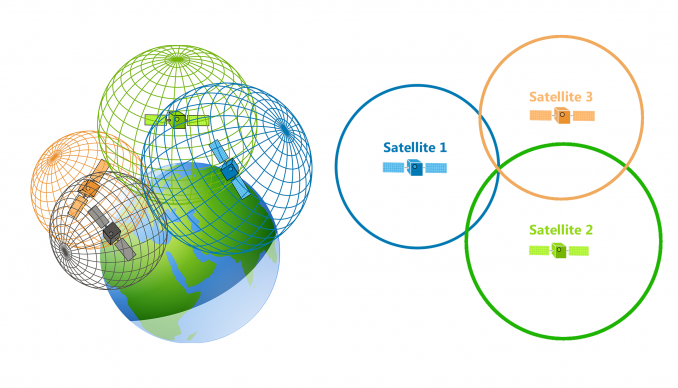
\includegraphics[width=0.7\textwidth]{pictures/multilateration/gps_multilateration.png}
    \caption{
        An example of how multilateration works in \ac{GNSS} in 2D and 3D~\protect\cite{gisgeography_how_2018}.
        It can be seen that 4 Satellites are needed to get a three-dimensional fix while only 3 are needed for a two-dimensional fix.
    }\label{pic:multilateration-gps-2d-3d-example}
\end{figure}

The correct term to use when using distances between an end device and multiple receivers to achieve a localization of the end device is \emph{multilateration}.
An example of this in \ac{GNSS} is shown in \cref{pic:multilateration-gps-2d-3d-example}.
A specific case of multilateration is \emph{trilateration}, which specifies three receivers to get the ranges from~\cite{ruiz_efficient_2013}.

\section{\acf{GNSS}}

\ac{GNSS} is a generic term for systems that use satellites orbiting the earth to determine the location of a device.
In everyday language, the term \ac{GPS} is often used as a synonym for \ac{GNSS}.
However, \ac{GPS} is only one of the several \ac{GNSS} systems that are currently in use.
\ac{GNSS} systems use multilateration to determine the location of end devices as explained in \cref{sec:multilateration-basics}.
\Cref{pic:multilateration-gps-2d-3d-example} shows an example of how this works with \ac{GNSS} satellites in 2D and 3D.
To determine the distance from the end device to the satellites, the time it takes for a signal to travel from the satellite to the end device is measured.
This approach is called \acf{ToA}.

\subsection{\acf{GPS}}

\ac{GPS} is the \ac{GNSS} system that is operated by the United States of America and is correctly called \emph{NAVSTAR \ac{GPS}}~\cite{department_of_defense_usa_gps_2020}.
The version of GPS the public has access to is called \acf{SPS}.
Additionally, there is the \acf{PPS} that is only available to the military and other authorized users~\cite{department_of_defense_usa_gps_2007}.

Using an iPhone 6, Merry and Bettinger measured the accuracy of \ac{GPS} to be between 7 and 13 meters in an urban environment~\cite{merry_smartphone_2019}.

\subsection{Other \acs{GNSS} systems}

There are several other \ac{GNSS} systems in use or in development by different countries.
For example, the Russian \acf{GLONASS} system, the European \acf{Galileo} system, the Chinese \acf{BDS} system, and the Indian \acf{IRNSS} system.

Most modern user devices such as smartphones support multiple \ac{GNSS} systems to improve the accuracy of the location determination.
For example, one of Samsung's most recent devices as of writing this thesis, the Galaxy S23 Ultra, supports \ac{GPS}, \ac{GLONASS}, \ac{Galileo}, and \ac{BDS}~\cite{gsmarena_samsung_2023}.

The \ac{LoRaWAN} nodes used in this thesis, as described in \cref{subsec:used-lora-nodes}, only use \ac{GPS} to determine their location.

\subsection{\acf{HDOP}}

% TODO: Explain HDOP and relevance to GPS accuracy
% relevance: only values with a low enough HDOP werer considered

\section{Localization techniques for usage with \acs{LoRaWAN}}\label{sec:lorawan-localization-techniques}

In the following sections, several concepts relating to localization in conjunction with \ac{LoRaWAN} will be explained.

\subsection{Multilateration}\label{sec:lorawan-multilateration}

As explained in \cref{sec:multilateration-basics}, multilateration uses the distance between a device and multiple receivers to determine the location of the end device.
However, while the theoretical concept of multilateration, as shown in \cref{pic:multilateration-gps-2d-3d-example} is simple, there are several challenges when applying it to real-world scenarios.
Distances measured between devices are often not accurate enough to determine the location of a device accurately.

\begin{figure}[htbp]
    \centering
    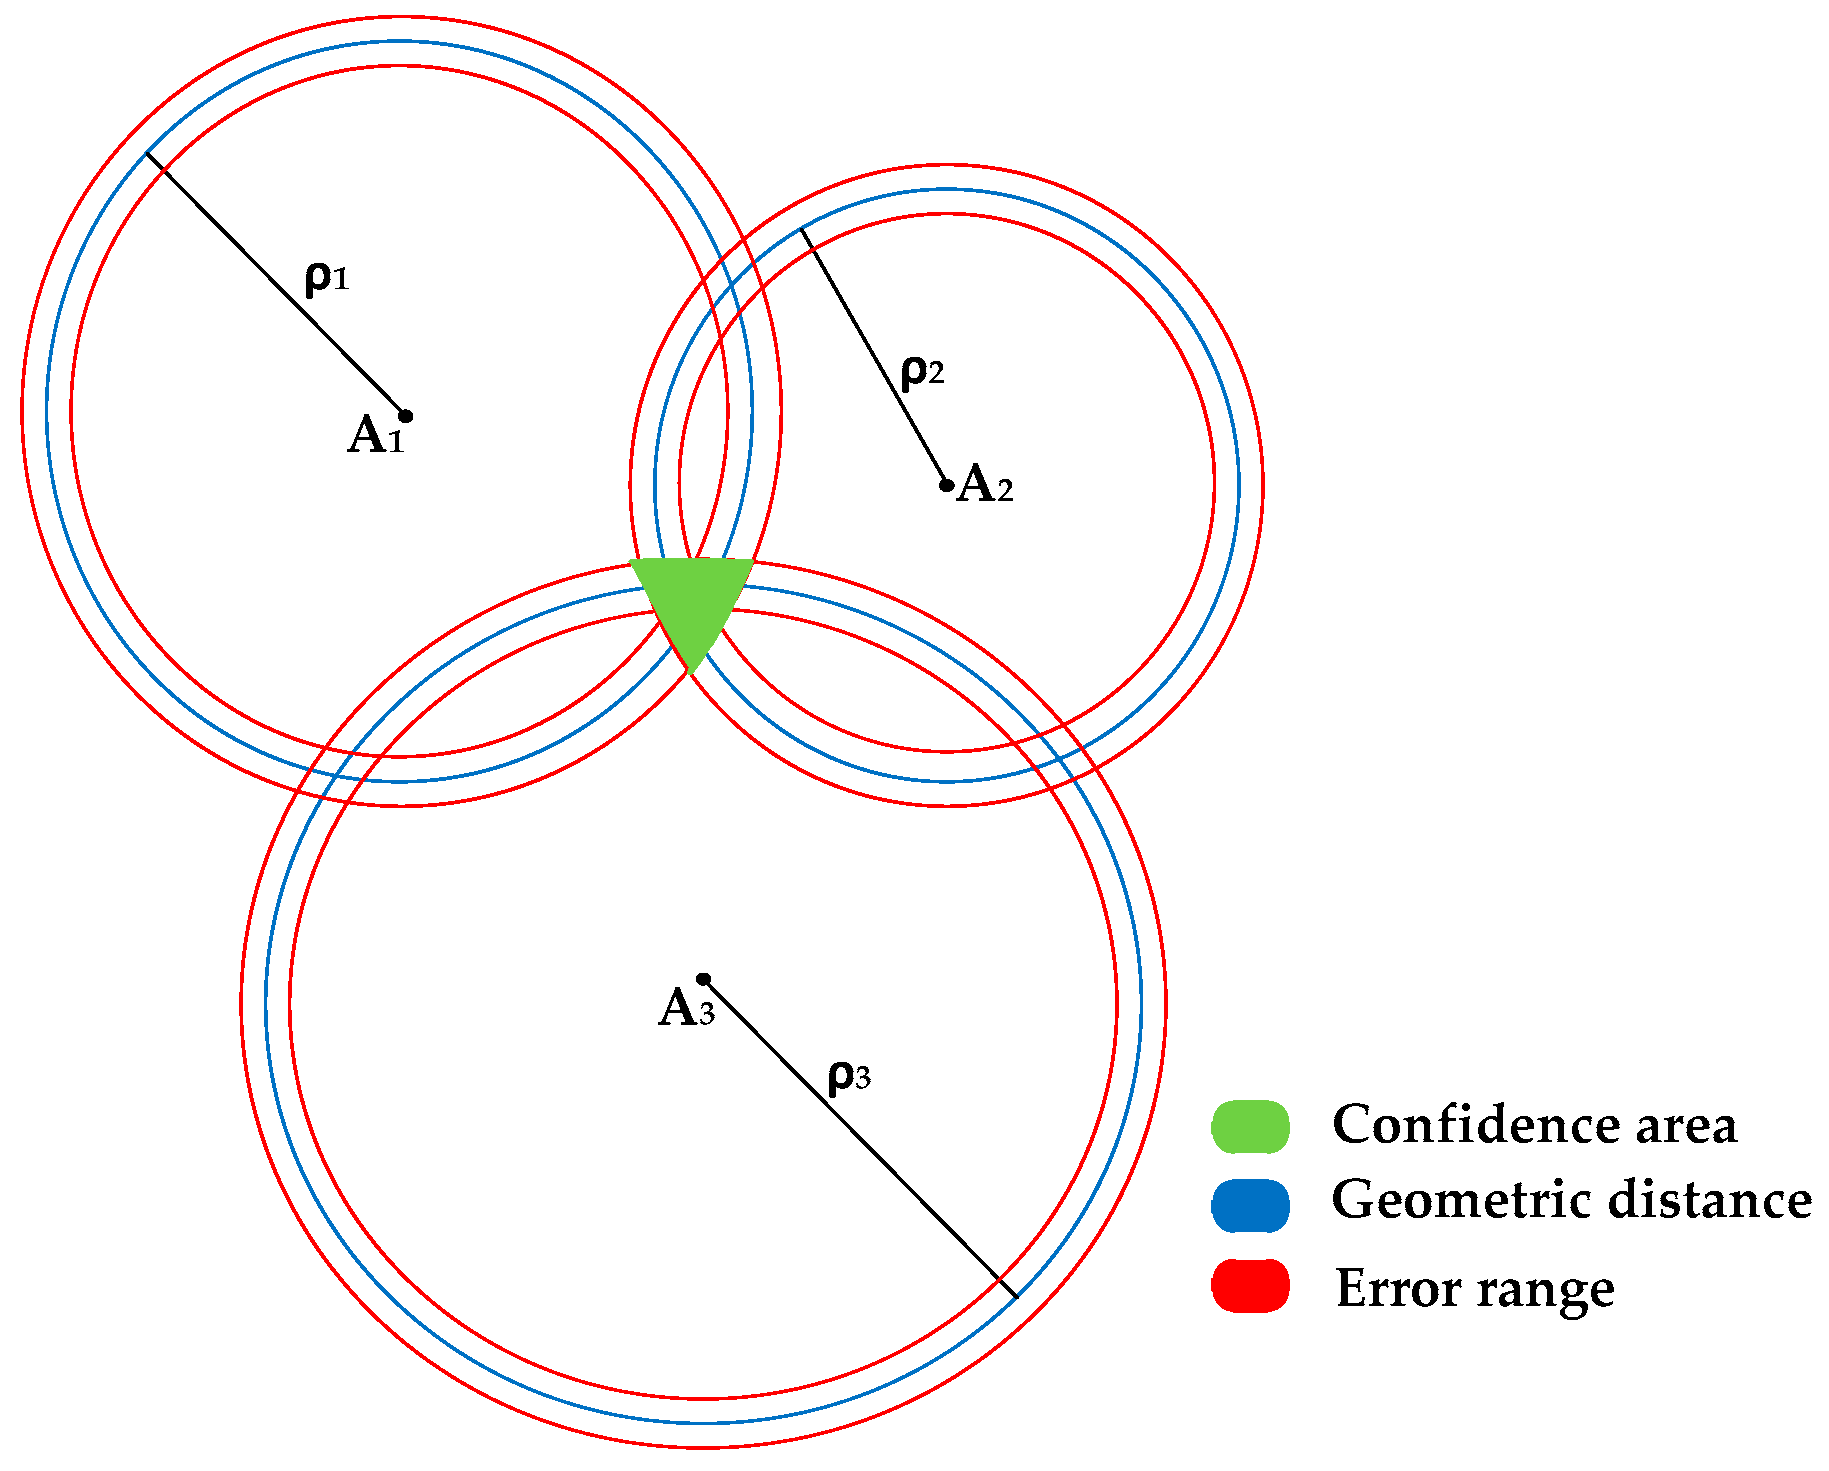
\includegraphics[width=0.7\textwidth]{pictures/multilateration/multilateration_error_ranges.png}
    \caption{
        An example of multilateration in 2D with error ranges.
        In contrast to the example shown in \cref{pic:multilateration-gps-2d-3d-example}, the margins of error can be seen as well as the non-definite margin of error around the estimated device position~\protect\cite{kapoor_novel_2016}.
    }\label{pic:multilateration-with-error-ranges-example}
\end{figure}

When dealing with such inaccuracies, the calculated position of the device often is calculated as not a single point but a range of possible positions.

\Cref{pic:multilateration-with-error-ranges-example} shows an example of this in 2D where the device's position is estimated to be in the area where the three annuli (``donuts'') overlap.
This does not result in a definite position of the device but rather a range of possible positions.
The size of this estimated localization range depends on the accuracy of the distance measurements.

The following sections will explain different methods of determining the distance between a device and a receiver.
However, as was just mentioned, the accuracy of these measurements is crucial for the accuracy of the actual localization.

\subsubsection{\acs{ToA}-based}\label{sec:toa-based-multilateration}

The \acf{ToA} based method uses the difference in the signal's time of arrival at the receiving stations.
In conjunction with the speed of light ($299792458\ \mathrm{m/s}$), this time difference can be used to calculate the distance between the receiving stations and the transmitting station~\cite{khalaf-allah_time_2015}.

\ac{ToA} is being used by radio location systems like \ac{GPS} to determine the position of a device by using Multilateration~\cite{department_of_defense_usa_gps_2020}.
For GPS, usually four or more satellites are required to determine the position of a device accurately.

\subsubsection{\acs{RSSI}-based}\label{sec:rssi-based-multilateration}

This method uses the \acf{RSSI} values that were explained in \cref{sec:rssi} to determine the distance between sender and receiver.
The distance between sender and receiver usually decreases in correlation with the measured \ac{RSSI} value.
However, as was mentioned in \cref{sec:multipath-propagation}, the \ac{RSSI} value can be also affected by other factors like obstacles and the environment.

These facts make \ac{RSSI}-based localization only work accurately in environments with little to no obstacles and thus a low amount of multipath propagation.
\Cref{sec:rssi-based-multilateration-implementation} will describe how this method was implemented in two different forms in this thesis.

\subsection{\acs{RSSI} Fingerprinting}\label{sec:rssi-fingerprinting}

Another method to locate devices is called fingerprinting~\cite{xia_indoor_2017}.
It uses a set of known device locations with their corresponding \ac{RSSI} values to locate devices based on the \ac{RSSI} values it receives from the surrounding receivers --- \ac{LoRaWAN} gateways, in this case.
The combination of an \ac{RSSI} value and the corresponding location is called a fingerprint.

When a new set of \ac{RSSI} values is recorded by a device, its \ac{RSSI} values are compared to the known \ac{DB} of known fingerprints.
The device's location can then be estimated by comparing the \ac{RSSI} values to the known fingerprints.
If multiple fingerprints match the \ac{RSSI} values, the device's location can be estimated by calculating the average or center of the locations of the matching fingerprints.

Using a multilayer perceptron \ac{ML} algorithm, Anagnostopoulos and Kalousis were able to achieve a median error of 204 meters using \ac{RSSI} fingerprinting~\cite{anagnostopoulos_reproducible_2019}.

This thesis will explore the use of \ac{RSSI} fingerprinting for \ac{LoRaWAN} localization in \cref{sec:fingerprinting-with-rssi-values}.
However, \ac{ML} was not used in this approach but only simpler similarity calculations.
Luckily, building a \ac{DB} of fingerprints for the use case explored in this thesis is rather simple, since the \ac{TTNM} \ac{API} already provides the necessary raw data as mentioned in \cref{sec:ttn-mapper-importance}.